\section{A Local Query Process for Algorithm 2 and its Complexity}\label{sec:query-process}

In this section, we define a query process to estimate the size of the output of \algtwo{}. 

In graph $H$ of \algtwo{}, each vertex corresponds to an edge in the original graph. More precisely, we make $K+2$ copies of each edge $(u, v)$ such that one of the copies corresponds to an edge occupying $(u^0, v^1)$, one for $(u^1, v^0)$, and $K$ for $(u^0, v^0)$. We use $G' = (V, E')$ to show the new graph with these parallel edges. During the course of \algtwo{}, two different edges that share the same endpoint and port cannot appear in the solution together. We use the following definition to formalize this notion.


\begin{definition}[Conflicting Pair of Edges]
Two edges $e, e' \in E'$ that share an endpoint $v$ are {\em conflicting} if both $e$ and $e'$ correspond to same port $v^i$ for $i \in \{0, 1\}$. We call $(e,e')$ a conflicting pair of edges.
\end{definition}

In order to estimate the size of the output of \algtwo{}, we define a vertex oracle that given a vertex $v$ and a permutation $\pi$ on $E'$, returns the degree of vertex $v$ in the output of \algtwo{}. These are akin to the query processes used before in the works of \cite{behnezhad2021,YoshidaYI09}, but are specific to our \algtwo{}.


\begin{algorithm}[H]
\caption{``vertex oracle'' $\VO(u, \pi)$ to determine the degree of vertex $u$ in $\RGMIS(G', \pi)$.}
\label{alg:vertexoracle}

	Let $e_1 = (u, v_1), \ldots, e_r = (u, v_r)$ be the edges incident to $u$ with $\pi(e_1) < \ldots < \pi(e_r)$.
	
	$d \leftarrow 0$
	
	\For{$i$ in $1 \ldots r$}{
		\lIf{$\EO(e_i, v_i, \pi) = \true$}{$d \leftarrow d+1$}
	}
	\Return $d$
\end{algorithm}

\begin{algorithm}[H]
\caption{``edge oracle'' $\EO(e, u, \pi)$ to determine an edge $e$ is in $\RGMIS(G', \pi)$. Also, $u$ must be an endpoint of $e$.}
\label{alg:edgeoracle}

    \lIf{$\EO(e, u, \pi)$ computed before}{\Return the computed result.}
    
	Let $e_1 = (u, v_1), \ldots, e_r = (u, v_r)$ be the edges incident to $e$ such that $\pi(e_1) < \ldots < \pi(e_r) < \pi(e)$. Also, $(e, e_i)$ is a conflicting pair for all $1 \leq i \leq r$.
	
	\For{$i$ in $1 \ldots r$}{
		\lIf{$\EO(e_i, v_i, \pi) =  \true$}{\Return \false}
	}
	
	\Return \true
\end{algorithm}


Note that in Line 2 of the \Cref{alg:edgeoracle} we only recursively call the function on edges that their label, conflict with edge $e$ since if other edges appear in the RMGIS subgraph, we can still have $e$ in the RGMIS subgraph. Before analyzing the query complexity of the vertex oracle, we prove the correctness of the vertex oracle.

\begin{claim}\label{clm:correctness-edge-oracle}
For any edge $e = (u, z) \in E'$ that is occupying ports $u^i$ and $z^j$, if $\EO(e, u, \pi)$ is called while computing $\VO(v, \pi)$, then $\EO(e, u, \pi) = \true$ iff $e \in \RGMIS(G', \pi)$.
\end{claim}
\begin{myproof}
We prove the claim using induction on ranking of edge $e$. Assume that the claim is true for all edges with ranking smaller than $\pi(e)$. If $\EO(e, u, \pi)$ is called by $\EO(e' = (w, z), z, \pi)$ or directly by $\VO(v, \pi)$, then by definition of \Cref{alg:edgeoracle} and \Cref{alg:vertexoracle}, all edges $e'' = (w', z)$ with $\pi(e'') < \pi(e')$ that are occupying $z^j$ are queried before $e'$ which means that none of them return \true{}. Hence, by induction hypothesis, none of the edges incident to $z$ that are occupying $z^j$ with lower rank are in the $\RGMIS(G', \pi)$. Moreover, $\EO(e, u, \pi)$ calls all incident edges to $u$ with lower rank that are occupying $u^i$ and return \true{} if none of them are in the $\RGMIS(G', \pi)$ by induction hypothesis. Therefore, $\EO(e, u, \pi) = \true$ iff $e \in \RGMIS(G', \pi)$.
\end{myproof}

\begin{claim}
Let $v \in V$ and $d$ be the output of $\VO(v, \pi)$. Then $d$ is equal to the degree of vertex $v$ in the subgraph outputted by $\RGMIS(G', \pi)$.
\end{claim}
\begin{myproof}
The observation follows by combining the fact that the vertex oracle queries edges in increasing order and \Cref{clm:correctness-edge-oracle}.
\end{myproof}


Let $T(v, \pi)$ denote the number of recursive calls to the edge oracle during the execution of $\VO(v, \pi)$.

\begin{theorem}\label{thm: query-complexity}
For a randomly chosen vertex $v$ and permutation $\pi$ on $E'$, we have that
\begin{align*}
    \E_{v, \pi}[T(v,\pi)] = O(\bar{d}\cdot \log^2 n)
\end{align*}
where $\bar{d}$ is the average degree of the graph $G$.
\end{theorem}

Let $Q(e, v, \pi)$ be the number of $\EO(e, \cdot, \pi)$ calls during the execution of $\VO(v, \pi)$. Moreover, let $Q(e, \pi)$ be the number of $\EO(e, \cdot, \pi)$ calls starting from any vertex. In other words, we have that $Q(e, \pi) = \sum_{v\in V}Q(e, v, \pi)$. 


\begin{observation}\label{obs: q-upperbound}
For every edge $e$ and permutation $\pi$, $Q(e, \pi) \leq O(n^2)$.
\end{observation}
\begin{myproof}
Let $e = \{x,y\}$. For a fixed vertex $u$, either the vertex oracle $\VO(u, \pi)$ queries the edge oracle for $e$ directly, or through some incident edge $e'$. Hence, the edge oracle of $e$ is called through at most $(K + 2)(\deg(x) - 1) + (K + 2)(\deg(y) - 1)$ of its incident edges ($K+2$ appears since each edge has $K + 2$ copies), which implies that $Q(e, u, \pi) \leq (2K + 4)(n - 1) + 1$. Therefore,
\begin{align*}
    Q(e, \pi) \leq \sum_{u\in V} Q(e, u, \pi) \leq n\left( (2K + 4)(n - 1) + 1 \right) \leq O(n^2).\qedhere
\end{align*}
\end{myproof}


The main contribution of this section is to show that the expected number of $\EO(e, \pi)$ calls over all permutations $\pi$ is $O(\log^2 n)$, which is formalized in the following lemma.

\begin{lemma}\label{lem: query-complexity}
For any edge $e \in E'$, we have $\E_\pi[Q(e, \cdot, \pi)] = O(\log^2 n)$.
\end{lemma}

Assuming the correctness of \Cref{lem: query-complexity}, we can complete the proof of \Cref{thm: query-complexity}.

\begin{myproof}[Proof of \Cref{thm: query-complexity}]
\begin{align*}
    \E_{v, \pi}[T(v, \pi)] = \frac{1}{n}\E_\pi\Big[\sum_{v\in V}T(v,\pi)\Big] & = \frac{1}{n}\E_\pi\Big[\sum_{v\in V}\sum_{e \in E'}Q(e,v,\pi)\Big] \\
    & = \frac{1}{n}\E_\pi\Big[\sum_{e \in E'}\sum_{v\in V}Q(e,v,\pi)\Big] = \frac{1}{n} \E_\pi\Big[\sum_{e \in E'} Q(e, \pi)\Big] \\ 
    & = \frac{1}{n} \sum_{e \in E'} \E_\pi[ Q(e, \pi)] = \frac{1}{n} \sum_{e \in E'} O(\log^2 n) \\
    & = \frac{1}{n} O(|E'|\cdot \log^2 n) = O(\bar{d}\cdot \log^2 n).\qedhere
\end{align*}
\end{myproof}

During the recursive calls to the edge oracle that starts from vertex $v$, the edges in the stack of recursive calls create a trail. 

\begin{observation}
Let $S = (e_1 = (v, u), e_2, \ldots, e_r)$ be the stack of recursive calls starting from vertex $v$. Then $(e_1, e_2, \ldots, e_r)$ is a trail in $G'$.
\end{observation}
\begin{myproof}
Since in Line 2 of \Cref{alg:edgeoracle}, edge oracle only queries incident edges, $(e_1, e_2, \ldots, e_r)$ is a walk. It remains to show that all edges are distinct. Suppose that $e_i = e_j$ for some $i < j$ which implies $\pi(e_i) = \pi(e_j)$. Since the edge oracle queries edges in decreasing order, we have $\pi(e_j) < \pi(e_i)$ which is a contradiction. 
\end{myproof}


We direct the edges of the trail from $v$ to the other endpoint. We call a trail that starts from $v$ on the graph with edge permutation $\pi$, a $(v,\pi)$-query-trail. For an edge $e = (x,y)$, let $\vec{e}$ denote the directed edge from $x$ to $y$ and $\cev{e}$ denote a directed edge from $y$ to $x$. 

\begin{observation}\label{obs:increasing_trail}
Let $\vec{P} = (\vec{e_1}, \vec{e_2}, \ldots, \vec{e_k})$ be a $(v, \pi)$-query-trail; then $\pi(e_1) > \pi(e_2) > \ldots > \pi(e_k)$.
\end{observation}
\begin{myproof}
During the answering whether an edge is in $\RGMIS(G',\pi)$, \Cref{alg:edgeoracle} recursively calls on edges with 
$\pi$ values lower than the value of the current edge. Therefore, the stack of recursive calls will be decreasing with respect to $\pi$ values.
\end{myproof}

Let $Q(\vec{e}, \pi) \subseteq Q(e, \pi)$ be the set of all query trails that end at $\vec{e}$ (with the same direction). In what follows, we obtain a bound for the query complexity for $\vec{e}$. We use this lemma to prove \Cref{lem: query-complexity}.


\begin{lemma}\label{lem: query-complexity-directed}
For any edge $e$, we have $\E_\pi[Q(\vec{e}, \pi)] = O(\log^2 n)$.
\end{lemma}

\begin{myproof}[Proof of \Cref{lem: query-complexity}]
Since $Q(e, \pi) = Q(\vec{e}, \pi) \cup Q(\cev{e}, \pi)$, by \Cref{lem: query-complexity-directed} we have 
\begin{align*}
\E_\pi[Q(e, \pi)] \leq \E_\pi[Q(\vec{e}, \pi)] + \E_\pi[Q(\cev{e}, \pi)] = O(\log^2 n) + O(\log^2 n) = O(\log^2 n). \qedhere
\end{align*}
\end{myproof}



Given a permutation $\pi$ and a trail $\vec{P}=(\vec{e_1}, \vec{e_2}, \ldots, \vec{e_k})$, we define $\phi(\pi, \vec{P})$ to be another permutation $\sigma$ over the edges such that:
\begin{align*}
    (\sigma(e_1), \sigma(e_2), \ldots, \sigma(e_{k-1}), \sigma(e_k)) \coloneqq (\pi(e_2), \pi&(e_3), \ldots, \pi(e_{k}), \pi(e_{1}))\\
    \pi(e') = \sigma(e') \quad\quad \forall e' \notin \vec{P}
\end{align*}

Given an edge $\vec{e}$, by using the above mapping function we can construct a bipartite graph $H$ with two parts $A$ and $B$ such that each part has $|E'|!$ vertices showing different permutations of edges. For a permutation $\pi \in A$ and a $(v,\pi)$-query-trail $\vec{P}$ that ends at $\vec{e}$ for some arbitrary vertex $v$, we connect $\pi$ in $A$ to $\phi(\pi, \vec{P})$ in $B$. Note that by construction of $H$, $\text{deg}(\pi_A) = Q(\vec{e},\pi_A)$ for all $\pi_A \in A$, since we have a unique edge for each query-trail that ends at $\vec{e}$ with permutation $\pi_A$. Hence, in order to prove \Cref{lem: query-complexity}, it is sufficient to prove that $\E_{\pi_A \sim A}[\text{deg}_H(\pi_A)]=O(\log^2 n)$. Let $\mathcal{Q}(\vec{e}, \pi)$ be the set of all query-trails for permutation $\pi$ that ends at $\vec{e}$. Let $\beta = c \log^2 n$ for some large $c$. We partition permutations into two sets of {\em likely} and {\em unlikely} permutations called $L$ and $U$ as follows:
\begin{align*}
    L \coloneqq \left\{\pi \in \Pi \Big\lvert \max_{\vec{P} \in \mathcal{Q}(\vec{e}, \pi)} |\vec{P}| \leq \beta \right\} \quad\quad U \coloneqq \Pi \setminus L.
\end{align*}

Likely permutations are those permutations that the longest query-trail ending at $\vec{e}$ has length at most $\beta$ and unlikely permutations are the remaining permutations. Let $A_L$ be the set of vertices corresponding to the likely permutations in $A$ and $A_U$ be the set of vertices corresponding to the unlikely permutations. The intuition behind this partitioning is that the set of unlikely permutations makes up a tiny fraction of all permutations which is formalized in \Cref{lem: few-long-trail}.

\begin{lemma}\label{lem: few-long-trail}
If $c$ is a large enough constant, then we have $|A_U| \leq |E'|! / n^2$.
\end{lemma}

Before proving \Cref{lem: few-long-trail}, we introduce the parallel implementation of the greedy maximal independent set.

\noindent\textbf{Parallel Randomized Greedy Maximal Independent Set:} Let $G$ be a graph and $\pi$ be a permutation over its edges. In each iteration, we pick all vertices whose rank is less than all their neighbors and remove all their neighbors. We denote the number of rounds in this algorithm until $G$ becomes empty as \textit{round complexity} and we show it with $\rho(G, \pi)$.

It is clear that the output of the parallel randomized greedy MIS is the same as $\RGMIS(G, \pi)$. We have the following known result about the round complexity of parallel randomized greedy MIS.


\begin{lemma}[{\cite[Theorem~3.5]{Blelloch12}}]\label{lem: parallel-RMGIS-rounds}
For a uniformly random chosen permutation $\pi$ over edges of $G$, we have $\rho(G, \pi) = O(\log^2 n)$, with probability of at least $1 - \frac{1}{n^2}$.
\end{lemma}


In order to use the above lemma, we need to show that for an unlikely permutation, the round complexity is large and therefore, small fraction of permutations are unlikely as a result of \Cref{lem: parallel-RMGIS-rounds}.

\begin{claim}\label{clm: large-round-complexity}
Let $\vec{P}$ be query-trail in $G'$ with permutation $\pi$. Then $\rho(G', \pi) \geq \lfloor \frac{|\vec{P}|}{2}\rfloor$.
\end{claim}
\begin{myproof}
Let $\vec{P} = (\vec{e_1}, \vec{e_2}, \ldots, \vec{e_k})$ be a query-trail. By \Cref{obs:increasing_trail}, we have $\pi(e_1) > \pi(e_2) > \ldots > \pi(e_k)$, where $e_k$ is the last edge on the trail. Let $\rho(e)$ show the round in which edge $e$ is deleted by the parallel algorithm. If we can show that for $i < k - 1$, $\rho(e_i) > \rho(e_{i+2})$, then we have that $\rho(e_2) \geq \lfloor \frac{k}{2}\rfloor$ which completes the proof. We prove it using a contradiction. Assume that $\rho(e_i) \leq \rho(e_{i+2})$ for some $1 < i < k - 1$. Note that $\rho(e_{i+1}) \geq \rho(e_i)$, otherwise, when $e_{i+1}$ is deleted from the graph, one of its corresponding ports that is shared with $e_i$ and $e_{i+2}$ was occupied which implies that at least one of $e_i$ and $e_{i+2}$ should be deleted at the same time. Hence, in round $\rho(e_i)$, edge $e_{i+1}$ is still present in the graph. Therefore, $e_i$ is not a local minimum in round $\rho(e_i)$ and is deleted due to presence of an edge $e'$ in the solution. Note that $e' \neq e_{i+1}$ since $e_{i+1}$ is not the minimum edge because $e_{i+2}$ is still in the graph. If $e'$ is only incident to $e_i$, $\EO(e_{i-1}, \cdot, \pi)$ should call $\EO(e', \cdot, \pi)$ before $\EO(e_i, \cdot, \pi)$ since $e'$ is the local minimum in round $\rho(e_i)$ and therefore $\pi(e') < \pi(e_i)$. If $e'$ is incident to both $e_i$ and $e_{i+1}$, $\EO(e_i, \cdot, \pi)$ should call $\EO(e', \cdot,\pi)$ before $\EO(e_{i+1}, \cdot,\pi)$ since $e'$ is local minimum at round $\rho(e_i)$ and therefore $\pi(e') < \pi(e_{i+1})$. In both cases, the edge oracle terminates and will not query edge $e_{i+2}$. Hence, the assumption that $\rho(e_i) \leq \rho(e_{i+2})$ leads to a contradiction and the proof is complete.
\end{myproof}

Now we are ready to prove \Cref{lem: few-long-trail}.

\begin{proof}[Proof of \Cref{lem: few-long-trail}]
For each unlikely permutation $\pi \in U$, there exists a query-trail of length larger than $\beta$. By \Cref{clm: large-round-complexity}, we have $\rho(G, \pi) \geq \lfloor \frac{\beta + 1}{2}\rfloor$. Since $\beta = c\log^2 n$, by choosing $c$ large enough and \Cref{lem: parallel-RMGIS-rounds}, we have that $|U|/|\Pi| \leq 1/n^2$. Therefore, $|U| \leq |E'|!/n^2$ which implies that $|A_U| \leq |E'|!/n^2$ since $A_U$ represents vertices that correspond to unlikely permutations.
\end{proof}


Next, we show that each vertex $\pi_B \in B$, has at most $\beta$ neighbors between likely permutations in part $A$ in bipartite graph $H$.

\begin{lemma}\label{lem: few-likely-neighbors}
Let $\pi_Y$ be a vertex in $Y$. Then $\pi_Y$ has most $\beta$ neighbors in $X_L$. 
\end{lemma}


Before proving this lemma, we show how we can prove \Cref{lem: query-complexity-directed} using \Cref{lem: few-long-trail} and \Cref{lem: few-likely-neighbors}.

\begin{proof}[Proof of \Cref{lem: query-complexity-directed}]
Note that by \Cref{obs: q-upperbound}, degree of each vertex $\pi_A \in A$ is at most $O(n^2)$. Combining \Cref{lem: few-long-trail}, we have
$$E(A_U, B) \leq |E'|! / n^2 \cdot O(n^2) \leq O\big(|E'|!).$$


Moreover, by \Cref{lem: few-likely-neighbors}, each vertex $\pi_B \in B$ has at most $O(\beta)$ neighbors in $A_L$. Since $H$ is a bipartite graph,  $E(A_L, B) \leq O(\beta)\cdot |A_L|$. Therefore, sum of degrees of all vertices in $A$ is at most 
\begin{align*}
    E(A_L, B) + E(A_U, B) \leq O(\beta)\cdot|A_L| + O(|E'|!) \leq O(\beta\cdot|E'|!).
\end{align*}

For a random vertex in $A$, the expected degree is $\frac{O(\beta \cdot |E'|!)}{|E'|!} = O(|E'|)$. Combining with $\beta = c\log^2 n$ and $\deg(\pi_A) = Q(\vec{e},\pi_A)$ completes the proof.
\end{proof}




The rest of this section, we prove \Cref{lem: few-likely-neighbors}. Before proving \Cref{lem: few-likely-neighbors}, we prove that if two different query-trails that are mapped to two different permutations of $A_L$ to $\pi_B \in B$ by $\phi$, the shorter query-trail must be subgraph of the longer one.

\begin{lemma}\label{lem:no-branch}
Let $\pi$ and $\pi'$ be two different permutations, and $\vec{P}$ and $\vec{P}'$ be $(v,\pi)$- and $(v',\pi')$-query-trail, respectively, that both end at edge $\vec{e}$. If $\phi(\pi,\vec{P})=\phi(\pi',\vec{P}')$ and $|\vec{P}| \geq |\vec{P}'|$, then $\vec{P}'$ is a subgraph of $\vec{P}$.
\end{lemma}

We prove this lemma by series of observations and claims. Let $\vec{P} = (\vec{e_k}, \ldots, \vec{e_1})$ and $\vec{P}'=(\vec{e_r}', \ldots, \vec{e_1}')$ such that $e=e_1=e_1'$. If $\vec{P}'$ is not a subgraph of $\vec{P}$, then it must branch after an edge $\vec{e_b}'$. This means that $\vec{e_i}=\vec{e_i}'$ for $i \leq b$ and $\vec{e_{b+1}} \neq \vec{e_{b+1}}'$. Note that $\vec{e_{b+1}}$ and $\vec{e_{b+1}}'$ can be copy of the same edge. 




\begin{observation}\label{obs:cons-conf}
Let $\pi$ be a random permutation over $E'$. For a $(u, \pi)$-query-trail, if $f$ and $f'$ are two consecutive edges in the trail, then $(f, f')$ is a conflicting pair.
\end{observation}
\begin{myproof}
Since the edge oracle calls $\EO(f', \cdot,\pi)$ in $\EO(f, \cdot, \pi)$, $(f, f')$ must be a conflicting pair.
\end{myproof}

\begin{observation}\label{obs:pair-conf}
Let $f_1, f_2, f_3$ be three different edges incident to some vertex $u$ and let $\pi$ be a random permutation over $E'$. Let $\vec{P_1}$ be a $(x, \pi)$-query-trail that calls $\EO(f_3, \cdot, \pi)$ in $\EO(f_1, \cdot, \pi)$. Also, let $\vec{P_2}$ be a $(y, \pi')$-query-trail that calls $\EO(f_3, \cdot, \pi')$ in $\EO(f_2, \cdot, \pi')$. Then $(f_1, f_2)$ is a conflicting pair.
\end{observation}
\begin{myproof}
By \Cref{obs:cons-conf}, $(f_1, f_3)$ is a conflicting pair. Assume that both $f_1$ and $f_3$ occupied port $u^i$. Moreover, since $(f_2, f_3)$ is a conflicting pair, then $f_2$ is also occupying $u^i$. Therefore, $(f_1, f_2)$ is a conflicting pair.
\end{myproof}


\begin{observation}\label{obs:equal_edge}
$\pi(e_b) = \pi'(e_{b+1})$.
\end{observation}
\begin{myproof}
Since $\vec{e_{b+1}}$ is not in $\vec{P}'$, we have that $\phi(\pi', \vec{P}')(e_{b+1})=\pi'(e_{b+1})$. Also, $\phi(\pi, \vec{P})(e_{b+1})=\pi(e_b)$ since $\phi(\pi, \vec{P})$ shifts edges of the trail $\vec{P}$ by one. Given that permutation $\phi(\pi, \vec{P})$ is equal to $\phi(\pi', \vec{P}')$, we have $\pi(e_b) = \pi'(e_{b+1})$.
\end{myproof}

Without loss of generality, we can assume that $\pi(e_b) \leq \pi'(e_b)$ since we did not make any difference between $\pi$ and $\pi'$ until this point.

\begin{observation}\label{obs:branch-begin}
$\pi'(e_{b+1}) < \pi'(e_b)$.
\end{observation}
\begin{myproof}
By combining \Cref{obs:equal_edge}, our assumption that $\pi(e_b) \leq \pi'(e_b)$, and the fact that $\pi'$ is a permutation, we have that $\pi'(e_{b+1}) < \pi'(e_b)$.
\end{myproof}

\begin{claim}\label{clm:equal-ranks}
If $\pi(f) < \pi(e_b)$ or $\pi'(f) < \pi(e_b)$ for some edge $\vec{f}$, then $\pi(f) = \pi'(f)$.
\end{claim}
\begin{myproof}
There are five different possible cases for $f$:
\begin{itemize}
    \item $\vec{f} \notin \vec{P} \cup \vec{P}'$: Since $\phi$ only changes the edge on the query-trail and $\phi(\pi, \vec{P})=\phi(\pi', \vec{P}')$, we have $\pi(f) = \pi'(f)$. 
    \item $\vec{f} \in \{\vec{e_1}, \ldots, \vec{e}_{b-1}\}$: Since $\phi(\pi, \vec{P})(e_{i+1}) = \phi(\pi', \vec{P}')(e_{i+1})$ for $1 \leq i < b$, we have $\pi(e_i) = \pi'(e_i)$. Hence, $\pi(f) = \pi'(f)$.
    \item $\vec{f}=\vec{e_b}$: In this case, condition $\pi(f) < \pi(e_b)$ does not hold since $\pi(f) = \pi(e_b)$. Also, $\pi'(f)=\pi'(e_b) \geq \pi(e_b)$. Therefore, condition $\pi'(f) < \pi(e_b)$ does not hold. 
    \item $\vec{f}\in \{\vec{e}_{b+1}, \ldots, \vec{e}_k\}$: By \Cref{obs:increasing_trail}, we have that $\pi(f) > \pi(e_b)$. Therefore, condition $\pi(f) < \pi(e_b)$ does not hold. Let $\vec{f}=\vec{e_i}$ for $i > b$. Since $\phi(\pi, \vec{P}) = \phi(\pi', \vec{P}')$, we have $\pi'(f) = \pi(e_{i-1}) \geq \pi(e_b)$. Therefore, none of the conditions in the claim statement holds.
    \item $\vec{f}\in \{\vec{e_{b+1}}', \ldots, \vec{e_r}'\}$: By \Cref{obs:increasing_trail}, we have that $\pi'(f) > \pi'(e_b)$. Combining by our assumption that $\pi'(e_b) \geq \pi(e_b)$, we have $\pi'(f) \geq \pi(e_b)$. Let $\vec{f}=\vec{e_i}'$ for $i > b$. Since $\phi(\pi, \vec{P}) = \phi(\pi', \vec{P}')$, we have that $\pi(f) = \pi'(e_{i-1}') \geq \pi'(e_b) \geq \pi(e_b)$. Therefore, none of the conditions in the claim statement holds.
\end{itemize}
The proof is thus complete.
\end{myproof}

\begin{claim}\label{clm:new-branch}
$e_{b+1} \in \RGMIS(G',\pi')$.
\end{claim}
\begin{myproof}
We prove the claim by contradiction. Assume that $e_{b+1} \notin \RGMIS(G',\pi')$. Hence, there exists an edge $f$ which is incident to $e_{b+1}$ such that $\pi'(f) < \pi'(e_{b+1})$. Thus, $\EO(e_{b+1}, \cdot, \pi')$ will recursively call $\EO(f, \cdot, \pi')$. Let $f$ be incident to $e_{i}$ and $e_{i+1}$ for $i \in \{b, b+1\}$. In the query-trail $\vec{P}$, $\EO(e_{i+1}, \cdot, \pi)$ calls $\EO(e_i, \cdot, \pi)$. Therefore, using the \Cref{obs:pair-conf}, we have that $(f,e_i)$ is a conflicting pair. Note that by \Cref{obs:equal_edge}, we have $\pi'(f) < \pi(e_b)$. Hence, $\pi(f) = \pi'(f) < \pi(e_b)$ by \Cref{clm:equal-ranks}. Since both permutations are identical for ranks lower than $\pi(e_b)$, edge $f$ must appear in $\RGMIS(G', \pi)$ and the query-trail $\vec{P}$ is not a valid query-trail since $\EO(e_i, \cdot, \pi)$ terminates upon calling $\EO(f, \cdot, \pi)$ (see \Cref{fig:branch}). 
\end{myproof}

\begin{figure}[htbp]
\begin{center}
  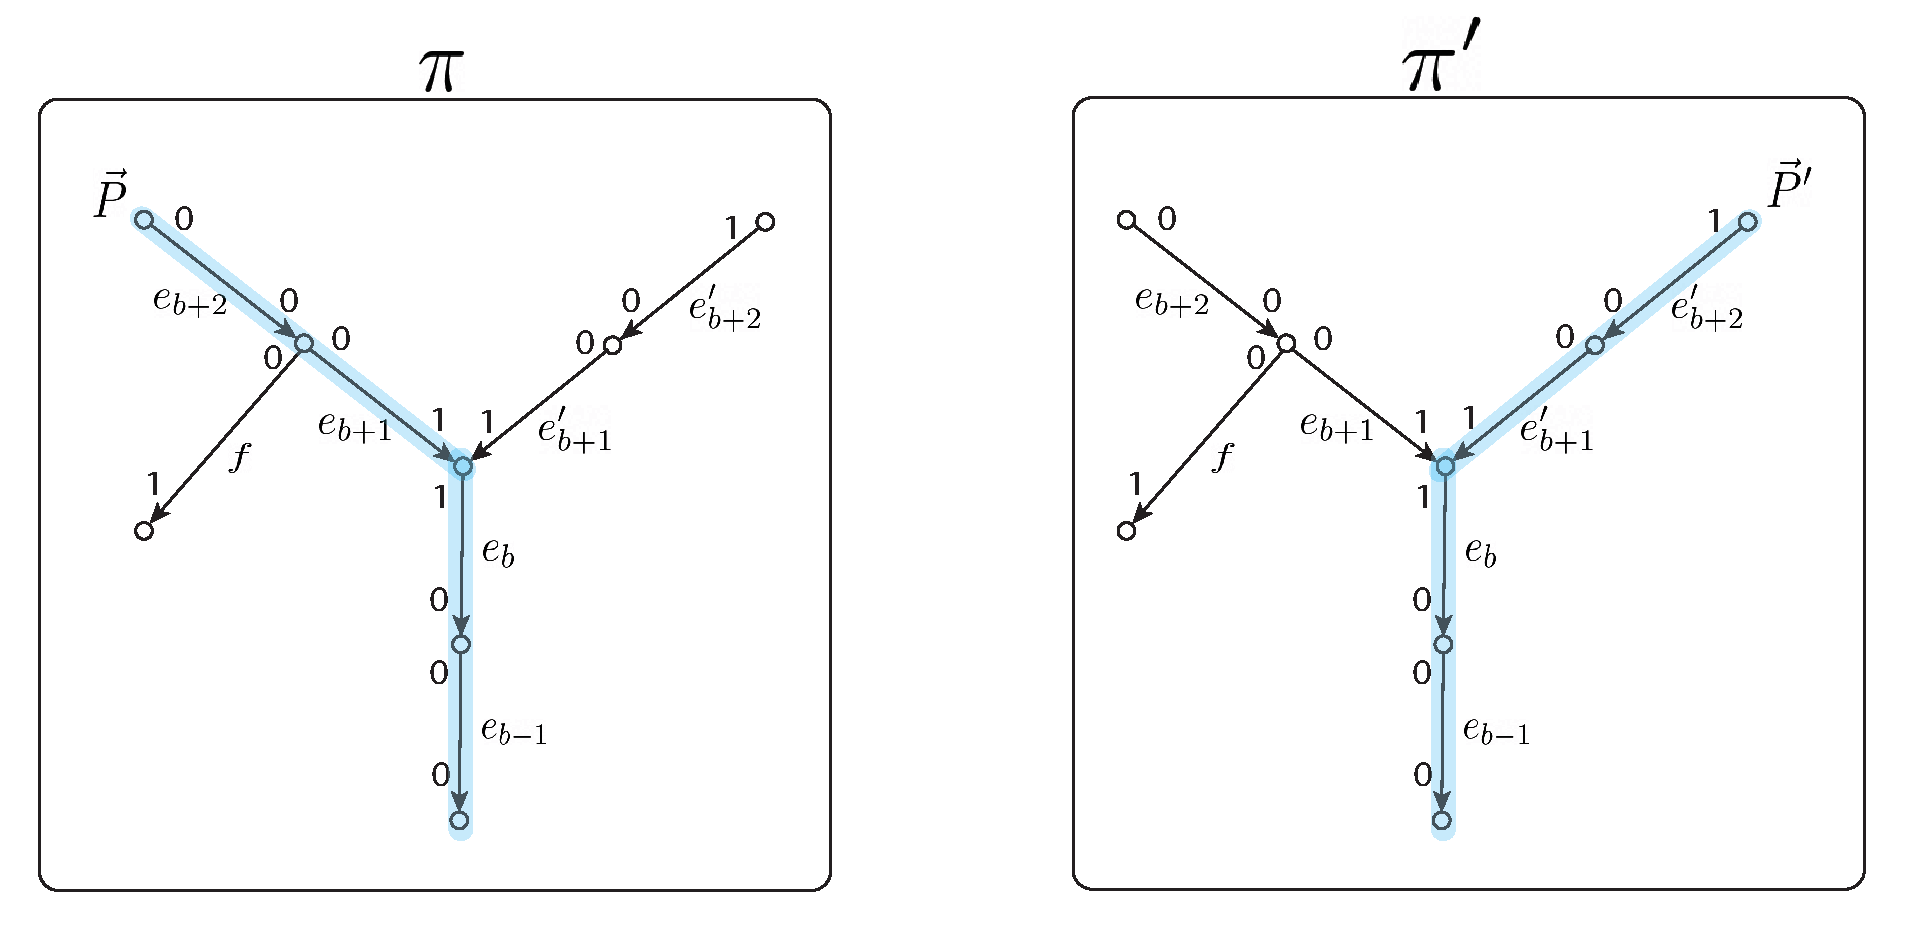
\includegraphics[scale=0.50]{fig/branch.pdf}
  \caption{Illustration of proof of \Cref{clm:new-branch}. The highlighted blue trails show query-trails $\vec{P}$ and $\vec{P}'$. Query-trail $\vec{P}$ is not valid since $\EO(e_i, \cdot, \pi)$ terminates upon calling $\EO(f, \cdot, \pi)$.}\label{fig:branch}
  \end{center}
\end{figure}


\begin{myproof}[Proof of \Cref{lem:no-branch}]
 We prove that query-trail $\vec{P}'$ is not a valid $(v, \pi')$-query-trail. Note that by \Cref{obs:branch-begin}, $\EO(e_{b+1}', \cdot, \pi')$ calls $\EO(e_{b+1}, \cdot, \pi')$ before $EO(e_b, \cdot, \pi')$. Thus, by \Cref{clm:new-branch}, $\EO(e_{b+1}, \cdot, \pi')$ will return \true{} and execution of $\EO(e_{b+1}', \cdot, \pi')$ terminates at this point. Therefore, query-trail $\vec{P}'$ is a subgraph of query-trail $\vec{P}$.
\end{myproof}


Now we are ready to complete the proof of \Cref{lem: few-likely-neighbors}.

\begin{proof}[Proof of \Cref{lem: few-likely-neighbors}]
For each edge between $\pi_A \in A_L$ and $\pi_B \in B$ in graph $H$, we write a label $\chi(\pi_A, \pi_B)$ on the edge which is equal to the length of the query-trail corresponding to this edge in $H$. By \Cref{lem:no-branch}, all the labels for edges of a fixed vertex $\pi_B \in B$ that are incident to $A_L$ should be different. Moreover, by the definition of likely permutations, all query-trails of permutation $A_L$ have length less than or equal to $\beta$. Thus, each vertex $\pi_B \in B$ has at most $\beta$ neighbors in $A_L$.
\end{proof}










\section{Our Estimator for Maximum Path Cover}\label{sec: disjoint-paths-estimate}
In this section, we use the oracle of the previous section to estimate the number of edges in the output of \algtwo{}. In \Cref{sec:query-process}, we provide a lower bound on the number of recursive calls to our local query process. Note that this bound does not necessarily imply the same running time algorithm. For example, if we generate the whole permutation over all copies of edges before running the algorithm, it takes $\Theta(m)$ which is no longer sublinear. Using by now standard ideas of the literature, we show in \Cref{sec:implementation} how we can implement the query process in almost the same running time (multiplied by a polylogarithmic factor) which is formalized in the following lemma.



\begin{restatable}{lemma}{oracleImplementation}\label{lem: implementation}
There exists a data structure that given a graph $G$ in the adjacency list format, (implicitly) fixes a random permutation $\pi$ over its edges. Then for any vertex $v$, the data structure returns the degree of vertex $v$ in the subgraph $P$ produced by \algtwo{} according to a random permutation $\pi$. Each query $v$ to the data structure is answered in $\Tilde{O}(T(v, \pi))$ time w.h.p. where $T(v, \pi)$ is as defined in \cref{sec:query-process}.
\end{restatable}


Note that in our local query process, we need access to the adjacency list of weight-one edges. So the challenge that arises here is how to estimate the size of the output of \algtwo{} in the adjacency matrix model. We present a reduction from adjacency matrix to adjacency list that appeared in the literature \cite{behnezhad2021}. In this reduction, each query to the adjacency list can be implemented with $O(1)$ queries to the adjacency matrix and still we are able to estimate the maximum path cover with some additive error.


Let $\gamma = 16Kn$. We construct a graph $\hat{G} = (V_{\hat{G}}, E_{\hat{G}})$ for weight-one edges of graph $G$ as follows:

\begin{itemize}
    \item $V_{\hat{G}}$ is the union of $V_1, V_2$ and $U_1, U_2, \ldots, U_n$ such that:
    \begin{itemize}
        \item $V_1$ and $V_2$ are two copies of the vertex set of the original graph $G$.
        \item $U_i$ is a vertex set of size $\gamma$ for each $i \in [n]$.
    \end{itemize}
    \item We define the edge set such that degree of each vertex is in $\{1, n, n + \gamma \}$:
    \begin{itemize}
        \item Degree of each vertex $v \in V_1$ is $n$. The $i$-th neighbor of $v$ is the $i$-th vertex in $V_1$ if $(v, i) \in E$, otherwise its $i$-th neighbor is the $i$-th vertex in $V_2$ for $i \leq n$. Note that graph $(V_1, E_H \cap (V_1 \times V_1))$ is isomorphic to $G$.
        \item Degree of each vertex $v \in V_2$ is $n + \gamma$. The $i$-th neighbor of $v$ is the $i$-th vertex in $V_2$ if $(v, i) \in E$, otherwise, its $i$-th neighbor is the $i$-th vertex in $V_1$ for $i \leq n$. For all $n < i \leq n + \gamma$, the $i$-th neighbor of $v$ is $i$-th vertex in $U_v$.
        \item Degree of each vertex $u \in U_i$ is one for $i \in [n]$. The only neighbor of $u$ is the $i$-th vertex of $V_2$.
    \end{itemize}
\end{itemize}

By the construction of $\hat{G}$, the only neighbor of $v \in \bigcup_{i=1}^n U_i$ can be determined without any query to the adjacency matrix. Also, the $i$-th neighbor of each vertex in $V_1 \cup V_2$ can be determined with one query.

\begin{observation}\label{obs: finding-neighbor}
For each vertex $v \in V_{\hat{G}}$ and $i \in [\deg_{\hat{G}}(v)]$, the $i$-th neighbor of vertex $v$ can be determined using at most one query to the adjacency matrix.
\end{observation}


Fix a vertex $v \in V_2$. When we run \algtwo{}, intuitively with high probability the first edge that is incident to $v$ and occupies port $v^0$ is between $v$ and $u \in U_v$. Furthermore, with high probability the first two edges that are incident to $v$ and occupies port $v^1$ are between $v$ and $u \in U_v$. A vertex $v \in V_2$ is an {\em abnormal} vertex if the above properties do not hold for $v$. Let $R \in V_2$ be the set of abnormal vertices. In the following observation, we show that for each vertex $v \in V_2 \setminus R$, all incident edges of $v$ in the output of \algtwo{} are between $v$ and vertices of $U_v$.


\begin{claim}\label{clm:abnormal-vertices-count}
$\E_\pi|R| \leq n/(4K)$
\end{claim}
\begin{myproof}
Fix a vertex $v \in V_2$. For a random permutation over copies of edges of $\hat{G}$, the first incident edge to $v$ that occupies port $v^0$ is between $v$ and $U_v$ with a probability of at least $\frac{(K + 1)\gamma}{(n + \gamma)(K+1)} \geq 1 - \frac{1}{8K}$. Moreover, the first two edges that occupy $v^1$ are between $v$ and $U_v$ with probability of at least $\frac{\gamma(\gamma - 1)}{(n+\gamma)(n+\gamma - 1)} \geq 1 - \frac{1}{8K}$. Since both events are independent, the probability of $v$ not being an abnormal vertex is at least
$$
\left(1 - \frac{1}{8K}\right)^2 \geq 1 - \frac{1}{4K}
,$$
which implies $\E_\pi|R| \leq n/(4K)$.
\end{myproof}


\begin{claim}\label{obs: good-vertices}
For each $v \in V_2 \setminus R$, all incident edges of $v$ in the output of \algtwo{} are between $v$ and vertices of $U_v$.
\end{claim}

\begin{myproof}
By definition of an abnormal vertex, let the first edge in the permutation incident to $v$ be between $v$ and $w \in U_v$ which occupies $v^0$. Since all copies of edges incident to $w$ are between $v$ and $w$, this edge will be added to the solution of \algtwo{}. Moreover, we know that the first two edges that are incident to $v$ and occupy port $v^1$ are between $v$ and $U_v$. Let these two edges be $(v, u_1)$ and $(v, u_2)$ where $u_1, u_2 \in U_v$. Note that the only way that $(v, u_1)$ is not added to the solution of \algtwo{} is when $u_1 = w$. In this case, since there is only one copy for each edge that occupied port $v^1$, then $u_2 \neq w$. Therefore, \algtwo{} adds $(v, u_2)$ to its output if it has not added $(v, u_1)$. Since both ports of $v$ are occupied in this case, all incident edges of $v$ in the output of \algtwo{} are between $v$ and vertices of $U_v$. 
\end{myproof}


\begin{observation}\label{obs: small-TSP-R}
Let $P$ be the output of \algtwo{} on $\hat{G}$. Then
$$
    \frac{1}{2} \rho(\hat{G}[V_1 \cup R]) \leq \E \left|P \cap (V_1 \cup R) \times (V_1 \cup R) \right| \leq (1+\frac{2}{K})\cdot \rho(\hat{G}[V_1 \cup R])
.$$
\end{observation}
\begin{myproof}
By \Cref{obs: good-vertices}, if we run \algtwo{} on $\hat{G}$, for any vertex $v \in V_2 \setminus R$, all incident edges of $v$ in the output are between $v$ and $U_v$. Hence, none of the edges between $V_2 \setminus R$ and $V_1 \cup R$ will be added to the output of \algtwo{}. Since, the permutation over edges of $V_1 \cup R$ is uniformly at random, by \Cref{clm: approximation-bound}, we obtain the claimed bound.
\end{myproof}


In the above sequence of observations, we show that there are few abnormal vertices in $V_2$, which implies that most of the incident edges to vertices of $V_1$ in the output of \algtwo{} are in $\hat{G}[V_1]$ (only those between $V_1$ and $R$ violate this property). Therefore, a natural way to estimate the number of edges in the output of \algtwo{} on $G$, is to estimate the number of edges in $\hat{G}[V_1]$ in the output of \algtwo{} on $\hat{G}$. With this intuition in mind, we need to bound the query complexity of the algorithm for a random vertex in $V_1$.


\begin{claim}\label{clm: v1query}
Let $v$ be a random vertex in $V_1$ and $\pi$ be a random permutation over edges of graph that is created by copying $E_{\hat{G}}$ according to \algtwo{}. Then
\begin{align*}
    \E_{v\sim V_1, \pi}[T(v, \pi)] = \tilde{O}(n).
\end{align*}
\end{claim}
\begin{myproof}
By \Cref{thm: query-complexity}, we have that
\begin{align*}
\E_{v\sim V_{\hat{G}}, \pi}[T(v, \pi)] = O(\frac{K\cdot |E_{\hat{G}}|}{|V_{\hat{G}}|}\cdot \log^2 |V_{\hat{G}}|).
\end{align*}
Summing over all vertices in $V_{\hat{G}}$, we obtain
\begin{align*}
    \sum_{v \in V_{\hat{G}}}\E_{\pi}[T(v, \pi)] = O(K \cdot |E_{\hat{G}}| \cdot \log^2 |V_{\hat{G}}|) = \tilde{O}(n^2),
\end{align*}
since $|V_{\hat{G}}| = O(n^2)$, $K = O(1/\epsilon)$, and $|E_{\hat{G}}| = O(n^2)$. Therefore, for a random vertex in $V_1$, we get
\begin{align*}
    \E_{v\sim V_1,\pi}[T(v, \pi)] \leq \left( \sum_{v \in V_{\hat{G}}}\E_{\pi}[T(v, \pi)] \right) / |V_1| = \tilde{O}(n). \qedhere
\end{align*}
\end{myproof}

\begin{algorithm}
\caption{Final algorithm for maximum path cover.}
\label{alg: disjoint-paths}
    Let $\hat{G} = (V_{\hat{G}}, E_{\hat{G}})$ as described above.

    $r \gets 192\cdot K^2 \cdot \log n$.
    
    Sample $r$ vertices $u_1, u_2, \ldots, u_r$ uniformly at random from $V_1$ with replacement.
    
    Sample $r$ ports $p_1, p_2, \ldots, p_r$ uniformly at random from $\{0, 1\}$.
    
    Run vertex oracle for each $u_i$ and let $X_i$ be the indicator if port $u_i^{p_i}$ is occupied with an edge in $\hat{G}[V_1]$ in output of \algtwo{}.
    

Let $X = \sum_{i \in [r]} X_i$ and $f = X/r$.

Let $\tilde{\rho} = \frac{K}{2(K + 2)}\cdot (f \cdot n - \frac{n}{4K})$.
    
\Return $\tilde{\rho}$
\end{algorithm}



\begin{lemma}\label{lem: error-bound}
Let $\tilde{\rho}$ be the output of \Cref{alg: disjoint-paths} on input graph $G$. With high probability, 
$$ \left(\frac{1}{2} - \frac{1}{K}\right)\cdot \rho(G) - \frac{n}{K} \leq \tilde{\rho} \leq \rho(G),$$
where $K$ is the parameter which is defined in \algtwo{}.
\end{lemma}
\begin{myproof}
Let $\hat{P}$ be the set of edges outputted by \algtwo{} on $\hat{G}$ with both endpoints in $V_1$. By \Cref{clm: approximation-bound}, we have that $\E|\hat{P}| \leq (1 + \frac{2}{K})\cdot\rho(G)$. Furthermore, by \Cref{clm:abnormal-vertices-count} and the fact that the degree of each vertex in the output of \algtwo{} is at most two, in the output of \algtwo{} on $\hat{G}[V_1 \cup R]$ we have at most $n/(2K)$ edges with one endpoint in $R$. Hence, combining with \Cref{clm: approximation-bound} and \Cref{obs: small-TSP-R} we get
\begin{align}\label{eq: phat-range}
    \frac{1}{2}\rho(G) - \frac{n}{2K} \leq \E|\hat{P}| \leq (1 + \frac{2}{K})\cdot \rho(G).
\end{align}
Since each edge in the output of \algtwo{} counted twice in \Cref{alg: disjoint-paths}, we have 
\begin{align*}
    \E[X_i] = \Pr[X_i = 1] = \frac{2 \E|\hat{P}|}{n},
\end{align*}
and,
\begin{align}\label{eq: X-expected2}
    \E[X] = \frac{2r \E|\hat{P}|}{n}.
\end{align}
Since $X$ is sum of $r$ independent random variables, by Chernoff bound (\Cref{prop:chernoff}) we get
\begin{align*}
    \Pr[|X - \E[X]| \leq \sqrt{6 \E[X] \log n}] \leq 2 \exp \left(-\frac{6 \E[X] \log n}{3 \E[X]} \right) = \frac{2}{n^2}.
\end{align*}
Combining $fn = Xn/r$ and the above bound, with probability of at least $1 - 2/n^2$ we have
\begin{align*}
    fn \in \frac{n(\E[X] \pm \sqrt{6 \E[X] \log n)}}{r} & = \frac{n\E[X]}{r} \pm \sqrt{\frac{6 n^2\E[X] \log n}{r^2}}\\
    & = 2\E|\hat{P}| \pm \sqrt{\frac{12n\E|\hat{P}| \log n}{r}} & (\text{By }(\ref{eq: X-expected2}))\\
    & = 2\E|\hat{P}| \pm \sqrt{\frac{n\E|\hat{P}|}{16K^2}} & (\text{Since } r = 192 \cdot K^2 \cdot \log n) \\
    & \in 2\E|\hat{P}| \pm \frac{n}{4K} & (\text{Since } \E|\hat{P}| \leq n).
\end{align*}
Since, $\tilde{\rho} = \frac{K}{2(K+2)}\cdot (f \cdot n - \frac{n}{4K})$, hence
\begin{align*}
    \frac{K}{K+2}\left(\E|\hat{P}| - \frac{n}{2K} \right) \leq \tilde{\rho} \leq \frac{K}{K+2} \cdot \E| \hat{P}|.
\end{align*}
Combining with (\ref{eq: phat-range}), implies the claimed bound.
\end{myproof}

\begin{theorem}\label{thm: disjoint-paths-algorithm}
Given an adjacency matrix access for input graph $G$, there exists a randomized algorithm that w.h.p. runs in $\widetilde{O}(n)$ time and  produces an estimate $\tilde{\rho}$, such that
$$
\left(\frac{1}{2} - \epsilon\right)\cdot\rho(G) - \epsilon n \leq \tilde{\rho} \leq \rho(G).
$$
\end{theorem}
\begin{myproof}
Let $K = \frac{1}{\epsilon}$ and $\tilde{\rho}$ be the output of \Cref{alg: disjoint-paths} on $G$. In \Cref{alg: disjoint-paths}, by combining \Cref{lem: implementation} and \Cref{clm: v1query}, the running time for each sample is $\tilde{O}(n)$. Since the number of samples is $r = 192K^2\log n$, and $K$ is a constant, the total running time of the algorithm is $\tilde{O}(n)$. Moreover, by \Cref{lem: error-bound} we get the approximation ratio in the statement.
\end{myproof}


\section{Our Estimator for (1,2)-TSP}
In this section, we use the algorithm for estimating the size of maximum path cover as a black box to estimate the size of (1,2)-TSP. First, note that if there is no Hamiltonian cycle with weight one edges of the graph, then the set of weight-one edges of the graph (1,2)-TSP is a solution for maximum path cover of graph $G$. Also, in the case that there exists a Hamiltonian cycle, then the size of maximum path cover is $n-1$. Moreover, if $P^*$ is the maximum path cover of a graph $G$, then it is possible to create a TSP by connecting these paths using edges with weight two. This intuition helps to formalize the following observation.

\begin{observation}\label{obs: bounding-TSP-with-DP}
Let $\tspsize{V}$ be the cost of (1,2)-TSP of graph $G = (V, E)$. Then, we have 
$$2n - \rho(G) - 1 \leq \tspsize{V} \leq 2n - \rho(G).$$
\end{observation}

Now we are ready to present the final algorithm for estimating (1,2)-TSP.


\begin{algorithm}
\caption{Final algorithm for (1,2)-TSP.}
\label{alg: 12tsp}

    Construct $\hat{G} = (V_{\hat{G}}, E_{\hat{G}})$ implicitly as desribed in \Cref{sec: disjoint-paths-estimate}.
    
    Let $\tilde{\rho}$ be the output of \Cref{alg: disjoint-paths} on $\hat{G}$.
    
    $\tilde{\tau} = 2n - \tilde{\rho}$
    
    \Return $\tilde{\tau}$
\end{algorithm}

\begin{lemma}\label{lem: 12tsp-approx}
Let $\tilde{\tau}$ be the output of \Cref{alg: 12tsp} and $\tspsize{V}$ be the cost of (1,2)-TSP of graph $G = (V, E)$. With high probability,
$$
\tspsize{V} \leq \tilde{\tau} \leq (\frac{3}{2} + \frac{4}{K})\cdot \tspsize{V},
$$
where $K$ is the parameter which is defined in \algtwo{}.
\end{lemma}
\begin{myproof}
By \Cref{obs: bounding-TSP-with-DP}, we have $2n - \rho(G) - 1 \leq \tspsize{V} \leq 2n - \rho(G)$. \Cref{alg: 12tsp} outputs $\tilde{\tau} = 2n - \tilde{\rho}$ as the estimate, where $\tilde{\rho}$ is the output of \Cref{alg: disjoint-paths}. Hence, by \Cref{lem: error-bound}, we have $2n - \tilde{\rho} \geq 2n - \rho(G)$. Also, by \Cref{lem: error-bound}, we have 
\begin{align*}
    2n - \tilde{\rho} & \leq 2n - (\frac{1}{2} - \frac{1}{K})\cdot \rho(G) + \frac{n}{K} \\
    & \leq 3n - \frac{3\rho(G)}{2} + \frac{4n}{K} - \frac{2\rho(G)}{K} - 1 & (\text{Since } \rho(G) < n)\\
    & \leq (\frac{3}{2} + \frac{4}{K})(2n - \rho(G) - 1) & (\text{Since } K \ll n) \\
    & \leq (\frac{3}{2} + \frac{4}{K})\cdot\tspsize{V} & (\text{Since } \tspsize{V} = 2n - \rho(G)),\\
\end{align*}
which completes the proof.
\end{myproof}

\begin{theorem}\label{thm: 12tsp}
Let $\tspsize{V}$ be the cost of (1,2)-TSP of graph $G = (V, E)$. For any $\epsilon > 0$, there exists an algorithm that estimate the cost of (1,2)-TSP, $\tilde{\tau}$, such that
$$
\tspsize{V} \leq \tilde{\tau} \leq (\frac{3}{2} + \epsilon)\cdot \tspsize{V},
$$
w.h.p in $\tilde{O}(n)$ running time.
\end{theorem}
\begin{myproof}
We choose $K = \frac{4}{\epsilon}$. By \Cref{lem: 12tsp-approx}, if $\tilde{\tau}$ is the output of \Cref{alg: 12tsp}, we get
\begin{align*}
    \tspsize{V} \leq \tilde{\tau} \leq (\frac{3}{2} + \epsilon)\cdot \tspsize{V}.
\end{align*}
Also, since the running time of \Cref{alg: 12tsp} is the same as the running time of \Cref{alg: disjoint-paths}, by \Cref{thm: disjoint-paths-algorithm}, the total running time is $\tilde{O}(n)$, which completes the proof.
\end{myproof}


\section{Our Estimator for Graphic TSP}\label{sec:graphic-TSP-minor}
In this section, we use our algorithm for estimating the size of maximum path cover to estimate the size of graphic TSP. In a recent work, Chen et al. \cite{chen2020} showed that it is possible to obtain a $(27/14)$-approximate algorithm for graphic TSP by estimating the matching size and the number of biconnected components in the graph. Since the size of graphic TSP is at most $2n$ (the cost of MST is $n-1$), they proved that if a graph has large matching and a few biconnected components, the cost of graphic TSP is significantly lower than $2n$. Since estimating the number of biconnected components is not an easy task in sublinear time, they use a proxy quantity that can be estimated in sublinear time.

We show that if we use our estimator for maximum path cover as a black-box instead of matching estimator in algorithm of \cite{chen2020}, we can improve the approximation ratio to $19/10$. Moreover, we show that we can estimate the number of bridges in $\tilde{O}(n)$. We exploit this estimation for further improvement to get a $11/6$-approximate algorithm for graphic TSP. 

Chen et al. \cite{chen2020} introduced the following definition of {\em bad vertex} as a proxy for estimating the number of biconnected components.

\begin{definition}[Bad Vertex]
We say a vertex $v \in V$ is a bad vertex, if one of the following holds:
\begin{itemize}
    \item degree of $v$ is 1,
    \item $v$ is a cut vertex with degree 2.
\end{itemize}
\end{definition}


In the following series of lemmas, we bound the cost of graphic TSP based on the size of maximum path cover and number of bad vertices. Almost all the steps of this part are similar to the algorithm for graphic TSP of \cite{chen2020} --- except the path cover subroutine that we use instead of maximal matching subroutine. We restate some of the useful lemmas to achieve the approximation bound that the black-box algorithm can get, and in the next subsection we improve this bound. First, we prove that if the size of the maximum path cover is small, the cost of graphic TSP is bounded away from $n$.

\begin{claim}\label{lem: lower-bound-path}
If the size of maximum path cover of graph $G$ is at most $\rho$, then the cost of graphic TSP is at least $2n - \rho$.  
\end{claim}
\begin{myproof}
Let $(v_0, v_2, \ldots, v_n = v_0)$ be the optimal graphic TSP of graph $G$. Note that the subgraph induced by weight-one edges of this cycle is a solution for path cover. Hence, at most $\rho$ edges in cycle $(v_0, v_2, \ldots, v_n = v_0)$ have weight one. All the remaining edges have a weight of at least two which implies the claimed bound.
\end{myproof}

Furthermore, the following lemma from \cite{chen2020}, provides a lower bound for a graphic TSP of graph in terms of number of bad vertices.

\begin{lemma}[{\cite[Lemma~2.8]{chen2020}}]\label{lem: lower-bound-bad-vertex}
If the number of bad vertices of graph $G$ is at least $\beta$, then the cost of graphic TSP is at least $n + \beta - 2$.
\end{lemma}


Chen et al. \cite{chen2020} showed that in a biconnected graph, if there exists a matching of large size, the cost of graphic TSP is significantly smaller than $2n$. 

\begin{lemma}[{\cite[Lemma~2.7]{chen2020}}]\label{lem: tsp-matching-bound}
Let $G$ be a graph and $M$ be a matching of $G$. Then the cost of graphic TSP is at most $2n - |M|$.
\end{lemma}

\begin{lemma}[{\cite[Lemma~2.11]{chen2020}}]\label{lem: non-bridge-matching}
Let $G$ be a graph and $M'$ be a matching that none of its edges is a bridge. Then the cost of graphic TSP is at most $2n - \frac{2}{3}|M'|$.
\end{lemma}

We now upper bound the cost of graphic TSP in terms of size of maximum path cover and number of bad vertices.

\begin{lemma}\label{lem:bound-path-cover-bad-vertices-tsp}
If the size of maximum path cover of graph $G$ is $\rho(G)$ and it has $\beta$ bad vertices, then the cost of graphic TSP is at most $2n - \frac{1}{5}(\rho(G) - 2\beta)$.
\end{lemma}
\begin{myproof}
Let $l$ be the number of non-trivial biconnected components and $M'$ be a maximum matching in graph $G$ that none of its edges is a bridge. Also, let $B$ be the number of bridges in $G$. By the proof of Lemma 2.9 of \cite{chen2020}, the cost of graphic TSP is at most $\min\{2n - \frac{2}{3}|M'|, 2n - l\}$. Note that there are at least $\rho(G) - B$ edges of the maximum path cover that are not bridge. Since all non-bridge edges of the maximum path cover are still union of several disjoint paths, there exists a matching with size of at least half of the edges of these paths. Hence, there exist a matching of size at least $\frac{1}{2}(\rho(G) - B)$. On the other hand, in the proof of the same lemma, they showed that $l \geq \frac{B}{2} - \beta$ which implies that the cost of graphic TSP is at most
\begin{align*}
\min\left\{2n - \frac{2}{3}|M'|, 2n - l\right\} \leq \min\left\{2n - \frac{1}{3}(\rho(G) - B), 2n - \frac{B}{2} + \beta\right\}.
\end{align*}
There are two possible cases:
\begin{itemize}
    \item If $B \leq \frac{2}{5}\rho(G) + \frac{6}{5}\beta$, then we have 
    \begin{align*}
        2n - \frac{1}{3}(\rho(G) - B) \leq 2n - \frac{1}{3}(\rho(G) - \frac{2}{5}\rho(G) - \frac{6}{5}\beta) = 2n - \frac{1}{5}(\rho(G) - 2\beta).
    \end{align*}
    \item If $B > \frac{2}{5}\rho(G) + \frac{6}{5}\beta$, then we have
    \begin{align*}
        2n - \frac{B}{2} + \beta \leq 2n - \frac{1}{5}\rho(G) - \frac{3}{5}\beta + \beta = 2n - \frac{1}{5}(\rho(G) - 2\beta).
    \end{align*}
\end{itemize}
Therefore, the cost of graphic TSP is at most
\begin{align*}
    \min\left\{2n - \frac{1}{3}(\rho(G) - B), 2n - \frac{B}{2} + \beta\right\} \leq 2n - \frac{1}{5}(\rho(G) - 2\beta). \qquad \qedhere
\end{align*}
\end{myproof}

Now we are ready to introduce the first algorithm for estimating the cost of graphic TSP, which uses our maximum path cover subroutine instead of the matching subroutine as a black-box. In \Cref{alg: graphic-tsp}, we first estimate the size of the maximum path cover and the number of bad vertices of the graph and report the graphic TSP cost in terms of the two estimations. The subroutine used for counting number of bad vertices is similar to the one in section 2.2 of \cite{chen2020}.

\begin{lemma}[\cite{chen2020}]\label{lem: bad-vertices-estimator}
Let $\beta$ be the number of bad vertices. For any constant $\epsilon > 0$, there exists an algorithm that w.h.p estimates the number of bad vertices $\tilde{\beta}$, such that $\beta \leq \tilde{\beta} \leq \beta + \epsilon n $, in $\tilde{O}(n)$ running time.
\end{lemma}

\begin{algorithm}
\caption{First algorithm for graphic TSP.}
\label{alg: graphic-tsp}
    Construct $\hat{G} = (V_{\hat{G}}, E_{\hat{G}})$ implicitly as desribed in \Cref{sec: disjoint-paths-estimate}.
    
    Let $\tilde{\rho}$ be the output of \Cref{alg: disjoint-paths} on $\hat{G}$.
    
    Let $\tilde{\beta}$ be the estimate of number of bad vertices.
    
    $\tilde{\tau} = 2n - \frac{1}{5}(\tilde{\rho} - 2\tilde{\beta})$
    
    \Return $\tilde{\tau}$
\end{algorithm}

\begin{lemma}\label{lem: graphic-tsp-approx1}
Let $\tilde{\tau}$ be the output of \Cref{alg: graphic-tsp} and $\tspsize{V}$ be the cost of graphic TSP of graph $G = (V, E)$. With high probability,
$$
\tspsize{V} \leq \tilde{\tau} \leq (\frac{19}{10} + \frac{1}{K})\cdot \tspsize{V},
$$
where $K$ is the parameter which is defined in \algtwo{}.
\end{lemma}





\begin{myproof}
Let $\beta$ be the number of bad vertices. By \Cref{lem: error-bound} and \Cref{lem: bad-vertices-estimator} $\tilde{\rho} \leq \rho(G)$ and $\beta \leq \tilde{\beta}$. Hence, we have $\tspsize{V} \leq \tilde{\tau}$ by \Cref{lem:bound-path-cover-bad-vertices-tsp}.

By \Cref{lem: error-bound} and \Cref{lem: bad-vertices-estimator}, we can estimate $\rho(G)$ and $\beta$ such that $\left(\frac{1}{2} - \frac{1}{K} \right)\rho(G) - \frac{n}{K} \leq \tilde{\rho}$ and $\tilde{\beta} \leq \beta + \frac{n}{K}$, if we choose $\epsilon = \frac{1}{K}$. Thus, we have
\begin{align*}
    \tilde{\tau} & \leq 2n - \frac{1}{5}\left( (\frac{1}{2} - \frac{1}{K})\cdot \rho(G) - \frac{n}{K} - 2(\beta + \frac{n}{K}) \right) \\
    & \leq 2n - \frac{1}{5}(\frac{\rho(G)}{2} - 2\beta) + \frac{4n}{5K}.& (\text{Since } \rho(G) \leq n). \\
\end{align*}
On the other hand, assume that the approximation ratio that the algorithm obtains is $\alpha + 1/K$ for some $\alpha \leq 2$. Thus, we get 
\begin{align*}
    (\alpha+ \frac{1}{K})\cdot \tau(V) & \geq \alpha\cdot\tau(V) + \frac{n}{K} & (\text{Since } \tau(V) \geq n) \\ 
    & \geq \alpha\cdot \max\{2n - \rho(G), n + \beta - 2\} + \frac{n}{K} & (\text{By  \Cref{lem: lower-bound-path}  and  \Cref{lem: lower-bound-bad-vertex}})\\
    & \geq \alpha\cdot \max\{2n - \rho(G), n + \beta\} + \frac{n}{K} - 4.
\end{align*}
So in order to show that $\tilde{\tau} \leq (\alpha + \frac{1}{K}) \cdot\tspsize{V}$, it is sufficient to show that 
\begin{align*}
2n - \frac{1}{5}(\frac{\rho(G)}{2} - 2\beta) + \frac{4n}{5K} \leq \alpha\cdot \max\{2n - \rho(G), n + \beta\} + \frac{n}{K} - 4.
\end{align*}
If $n$ is large enough, then we have $\frac{4n}{5K} \leq \frac{n}{K} - 4$, which implies that we need to prove
\begin{align*}
    2n - \frac{1}{5}(\frac{\rho(G)}{2} - 2\beta) \leq \alpha\cdot \max\{2n - \rho(G), n + \beta\}.
\end{align*}
Now, let $\rho(G) = xn$ and $\beta = yn$ for $0 \leq x \leq 1$ and $ 0\leq y \leq 1$. To obtain $\alpha$, it suffices to solve the following program
\begin{align*}
\begin{array}{ll@{}ll}
\text{maximize}  & \alpha \\
\vspace{5px}\text{subject to}& \frac{2 - \frac{1}{5}(\frac{x}{2} - 2y)}{\max\{2-x, 1+y\}} \leq \alpha,\\
                & 0\leq x \leq 1,\\
                 & 0\leq y \leq 1.
\end{array}
\end{align*}
This is a constant size program that can be easily solved; the solution is $19/10$.\footnote{See e.g. this WolframAlpha \href{https://www.wolframalpha.com/input?i=Maximize\%5B\%282-1\%2F5*\%28x\%2F2+-+2y\%29\%29+\%2F+Max\%5B2-x\%2C+1\%2By\%5D\%2C+\%7B0\%3C\%3D+x+\%3C\%3D1\%2C+0\%3C\%3Dy\%3C\%3D1\%7D\%2C+\%7Bx\%2Cy\%7D\%5D}{link}.} This completes the proof.
\end{myproof}



\begin{theorem}\label{thm: graphic-tsp}
Let $\tau(V)$ be the cost of graphic TSP of graph $G = (V, E)$. For any $\epsilon > 0$, there exists an algorithm that estimate the cost of graphic TSP, $\tilde{\tau}$, such that
$$
\tau(V) \leq \tilde{\tau} \leq (\frac{19}{10} + \epsilon) \cdot \tau(V),
$$
w.h.p in $\tilde{O}(n)$ running time.
\end{theorem}
\begin{myproof}
Let $\tilde{\tau}$ be the output of \Cref{alg: graphic-tsp}. If we choose $K = \frac{1}{\epsilon}$, then by \Cref{lem: graphic-tsp-approx1}, we have 
$$
\tau(V) \leq \tilde{\tau} \leq (\frac{19}{10} + \epsilon) \cdot \tau(V).
$$
Also, by \Cref{thm: disjoint-paths-algorithm} and \Cref{lem: bad-vertices-estimator}, estimating $\tilde{\rho}$ and $\tilde{\beta}$ can be done in $\tilde{O}(n)$ time.
\end{myproof}


\section{Further Improvement for Graphic TSP}\label{sec:graphic-TSP-major}
In this section, we design an algorithm to estimate the number of bridges in given graph $G$. Equipped with this tool, we are able to estimate the number of non-bridge edges in the path cover which helps to improve the approximation ratio. Before describing the techniques for estimating the number of bridges, we prove the following lemma that provides a lower bound on the cost of graphic TSP based on the number of bridges in the graph.

\begin{claim}\label{lem:brdige-lower-bound}
If the number of bridges in the graph $G$ is at least $B$, then the cost of the graphic TSP is at least $n + B$.
\end{claim}
\begin{myproof}
Since the metric in the graphic TSP is corresponding to the shortest path distances in graph $G$, then a TSP tour is corresponding to a closed walk that contains all vertices. Thus, each bridge should be crossed at least two times in this walk in order for the walk to be closed and cover all vertices. Therefore, the cost of graphic TSP is at least $n + B$.
\end{myproof}


In the following series of lemmas, first, we prove that there are a few bridges that both of their endpoints have a high degree and then we show an efficient way to estimate the number of bridges that have at least one endpoint with a low degree. Combining the above arguments is the main idea to estimate the number of bridges.


\begin{lemma}\label{lem:few-high-deg-bridges}
For any integer $c \geq 2$, there exists at most $\frac{2n}{c}$ bridges that both of their endpoints have a degree larger than $c$. 
\end{lemma}
\begin{myproof}
Let $\mathcal{B}$ be the set of bridges that both of their endpoints have a degree larger than $c$. We construct a tree, $T_\mathcal{B}$, with edge set equal to $\mathcal{B}$ such that each vertex of $T_\mathcal{B}$ corresponds to a component of vertices that are compressed to a single vertex. We construct $T_\mathcal{B}$ iteratively. In the beginning, we consider the bridge-block tree of the original graph. In each step, if there exists a bridge $e = (u,v)$ (note that $u$ and $v$ are vertices of the tree and corresponding to a set of vertices of the original graph) such that at least one of its endpoints has a degree less than or equal to $c$, we merge $u$ with $v$ and add all edges of $u$ to $v$. We continue this process until there is no bridge with an endpoint of degree less than or equal to $c$.

Now, we prove that $|\mathcal{B}| \leq \frac{2n}{c}$. Let $x_v$ denote the number of vertices in the original graph that are compressed to vertex $v \in T_\mathcal{B}$. We remove vertices of $T_\mathcal{B}$ one by one until there is no vertex in the tree. At each step, we remove a leaf $v \in T_\mathcal{B}$ and at the end when only one vertex is remaining, we remove that vertex. Let $y_v$ be the number of incident edges to $v$ in $T_\mathcal{B}$ that are removed before removing $v$. At the time that we are removing leaf $v$, we have $x_v + y_v + 1\geq c + 1$, since the endpoint of the leaf that is the component of $v$ has at most $x_v$ incident edges in the same component in the original graph, $y_v$ incident edges to the other components that are removed before, and there is only one remaining incident edge to other components (the other endpoint of the leaf). Thus, 
\begin{align}\label{eq:x-bound}
    \sum_{v \in T_\mathcal{B}} x_v \geq \sum_{v \in T_\mathcal{B}} (c - y_v) = (|\mathcal{B}| + 1)c - \sum_{v \in T_\mathcal{B}}y_v.
\end{align}

Since vertices of each component are disjoint, we have $\sum_{v \in T_\mathcal{B}} x_v = n$. Moreover, we have $\sum_{v \in T_\mathcal{B}} y_v = |\mathcal{B}|$ since each edge of $\mathcal{B}$ counted when one of its endpoints is deleted from the tree. Combining above bounds and inequality (\ref{eq:x-bound}), we have
\begin{align*}
    n = \sum_{v \in T_\mathcal{B}} x_v \geq  (|\mathcal{B}| + 1)c - |\mathcal{B}|
\end{align*}
Therefore,
\begin{align*}
    |\mathcal{B}| \leq \frac{n - c}{c - 1} \leq \frac{2n}{c},
\end{align*}
where the last inequality holds for sufficiently large $n$.
\end{myproof}

\begin{lemma}\label{lem:test-bridge}
Let $c \geq 2$ be a constant and $u$ is a vertex such that $\deg(u) \leq c$. Then we can test if each of incident edges of $u$ is a bridge in  $O(n)$ total running time.
\end{lemma}
\begin{myproof}
We can query all neighbors of $u$ in $O(n)$. Assume that $\{v_1, v_2, \ldots, v_r\}$ are neighbors of $u$ for $r \leq c$. Now we divide the vertices of the graph except $u$ into $r$ sets $V_1, V_2, \ldots, V_r$. For each vertex $w \neq u$, we query the distance of $w$ to all $\{v_1, v_2, \ldots, v_r\}$. Let $v_i$ be the closest one to $w$ (if there is a tie, choose the one with the lowest index). Then we put $w$ in $V_i$. Note that since $c$ is a constant and $r \leq c$, this step can be done in $O(n)$.


Now we claim that $(u, v_j)$ is a bridge iff the following conditions hold:
\begin{itemize}
    \item For each $w \in V_j$ and $i \neq j$, $d(w, v_i) - d(w, v_j) = 2.$
    \item For each $w \in V_i$ such that $i \neq j$, $d(w, v_j) - d(w, v_i) = 2.$
\end{itemize}

Suppose that $e = (u, v_j)$ is a bridge. Since removing $e$ creates two connected components $C_u$ and $C_{v_j}$, all vertices in $C_{v_j}$ (resp. $C_u$) have a closer distance to $v_j$ (resp. $u$). In other words, all shortest paths between $w \in V_j$ to $v_i$ for $i \neq j$, cross edges $(v_j,u)$ and $(u, v_i)$. In addition, all the shortest paths between $w \in V_i$ and $v_j$ for $i \neq j$, cross edges $(v_j,u)$ and $(u, v_i)$. Therefore, both conditions hold.

Now suppose that $e = (u, v_j)$ is not a bridge. In this case, there must be an edge between $V_j$ and at least one of $V_i$ as otherwise, $V_j$ will be disconnected from the rest of the graph by removing $e$. Without loss of generality, assume that this edge is $(w, w')$ such that $w \in V_j$, $w' \in V_i$, and $i \neq j$. Also, w.l.o.g., we assume $d(w,v_j) \leq d(w', v_i)$. Since there is an edge between $w$ and $w'$, we have $d(w', v_j) \leq 1 + d(w, v_j) \leq 1 + d(w', v_i)$, which contradicts the conditions.

To test whether the conditions hold, we need to query the distance of each vertex to all $\{v_0, v_1, \ldots, v_r\}$ which can be done in $O(n)$ in total since $r$ is a constant.
\end{myproof}


\begin{lemma}\label{lem:bridge-estimator}
Let $B$ be the number of bridges in graph $G$. For any $\epsilon > 0$, there exists an algorithm that outputs an estimate $\tilde{B}$ in $\tilde{O}(n)$ such that $B \leq \tilde{B} \leq B + \epsilon n$.
\end{lemma}
\begin{myproof}
By \Cref{lem:few-high-deg-bridges}, there are at most $\frac{\epsilon n}{2}$ bridges with both endpoints have degree larger than $\frac{4}{\epsilon}$. Let $\hat{B}$ be the number of bridges that at least one of their endpoint has degree of at most $\frac{4}{\epsilon}$. Thus,
\begin{align}\label{eq:b-range}
    B - \frac{\epsilon n}{2} \leq \hat{B} \leq B.
\end{align}

We sample $r = 256\cdot \epsilon^{-4} \cdot \log n$ vertices uniformly at random with replacement. Let $u$ be the $i$-th sampled vertex. If the degree of the vertex is larger than $\frac{4}{\epsilon}$, we let $X_i = 0$. Otherwise, let $\{v_1, v_2, \ldots, v_k\}$ be the neighbors of $u$ where $k \leq \frac{4}{\epsilon}$. By \Cref{lem:test-bridge}, we can test if each of the incident edges of $u$ is a bridge in $O(n)$ total running time. For each edge $(u, v_j)$ if $\deg(u) < \deg(v_j)$ or $\deg(u) = \deg(v_j)$ and index of $u$ is smaller than $v_j$, we test if the edge is a bridge or not. Let $X_i$ show the number of successful tests for incident edges of $u$. Note that in the above algorithm, each bridge with low-degree endpoints only counted once. 

Let $\bar{X} = (\sum_{i}^{r} X_i) / r$ and $n\bar{X} + \frac{3\epsilon n}{4}$ be our final estimate of the number of bridges. Hence, $\E[\bar{X}] = \hat{B}/n$. Since $\bar{X}$ is the average of $r$ independent random variables such that $0 \leq X_i \leq 4/\epsilon$, by Hoeffding's inequality (\Cref{prop:hoeffding}) we obtain
\begin{align*}
    \Pr\left[\left|\bar{X} - \E[\bar{X}]\right| \geq \frac{\epsilon}{4}\right] \leq 2\exp\left(-\frac{r\epsilon^4}{128}\right) = \frac{2}{n^2},
\end{align*}
where the last inequality follows from $r = 256\cdot \epsilon^{-4} \cdot \log n$. Therefore, with probability of $1 - \frac{2}{n^2}$,
\begin{align*}
    n\bar{X} & \in n\E[\bar{X}] \pm \frac{n\epsilon}{4}\\
    & = \hat{B} \pm \frac{n\epsilon}{4} & (\text{Since } \E[\bar{X}] = \hat{B}/n).
\end{align*}
Combining above range and inequality (\ref{eq:b-range}), we get
\begin{align*}
    B\leq n\bar{X} + \frac{3\epsilon n}{4} \leq B + \epsilon n.
\end{align*}
Since the number of sampled vertices is $r = 256\cdot \epsilon^{-4} \cdot \log n$, the total running time is $\tilde{O}(n)$.
\end{myproof}

Now we are ready to introduce the improved algorithm for graphic TSP.

\begin{algorithm}
\caption{Improved algorithm for graphic TSP.}
\label{alg: graphic-tsp2}
    Construct $\hat{G} = (V_{\hat{G}}, E_{\hat{G}})$ implicitly as described in \Cref{sec: disjoint-paths-estimate}.
    
    Let $\tilde{\rho}$ be the output of \Cref{alg: disjoint-paths} on $\hat{G}$.
    
    Let $\tilde{B}$ be the estimate of the number of bridges. 
    
    $\tilde{\tau} = 2n - \frac{1}{3}(\tilde{\rho} - \tilde{B})$
    
    \Return $\tilde{\tau}$
\end{algorithm}


\begin{lemma}\label{lem: graphic-tsp-approx2}
Let $\tilde{\tau}$ be the output of \Cref{alg: graphic-tsp2} and $\tspsize{V}$ be the cost of graphic TSP of graph $G = (V, E)$. With high probability,
$$
\tspsize{V} \leq \tilde{\tau} \leq (\frac{11}{6} + \frac{1}{K}) \cdot \tspsize{V},
$$
where $K$ is the parameter which is defined in \algtwo{}.
\end{lemma}
\begin{myproof}
Let $\rho(G)$ be the size of maximum path cover and $B$ be the number of bridges in the graph. There are at least $\rho(G) - B$ edges of maximum path cover that are not bridge. These edges construct disjoint paths which implies there exists a matching of size $\frac{1}{2}(\rho(G) - B)$ that none of its edges is a bridge. Hence, by \Cref{lem: non-bridge-matching}, the cost of graphic TSP is at most $2n - \frac{1}{3}(\rho(G) - B)$. Therefore, since $\tilde{\rho} \leq \rho(G)$ and $B \leq \tilde{B}$, we get $\tspsize{V} \leq \tilde{\tau}$.

By \Cref{lem: error-bound} and \Cref{lem:bridge-estimator}, we have $\left(\frac{1}{2} - \frac{1}{K} \right)\cdot\rho(G) - \frac{n}{K}\leq \tilde{\rho}$ and $\tilde{B} \leq B + \frac{n}{K}$ which implies
\begin{align*}
    \tilde{\tau} & \leq 2n - \frac{1}{3}\left( (\frac{1}{2} - \frac{1}{K})\cdot\rho(G) - (B + \frac{n}{K}) \right) \\
    & \leq 2n - \frac{1}{3}(\frac{\rho(G)}{2} - B) + \frac{2n}{K} & (\text{Since } \rho(G) \leq n).
\end{align*}
Also, assume that the approximation ratio that the algorithm obtains is $\alpha + 2/K$ for some $\alpha \leq 2$. Thus,
\begin{align*}
    (\alpha + \frac{2}{K}) \cdot \tspsize{V} & \geq \alpha \cdot \tspsize{V} + \frac{2n}{K} & (\text{Since } \tspsize{V} \geq n) \\ 
    & \geq \alpha\cdot \max\{2n - \rho(G), n + B\} + \frac{2n}{K} & (\text{By \Cref{lem: lower-bound-path}  and  \Cref{lem:brdige-lower-bound}}).
\end{align*}
Therefore, to show that $(\alpha + \frac{1}{K})\cdot\tspsize{V} \geq \tilde{\tau}$, it is sufficient to show 
\begin{align*}
    2n - \frac{1}{3}(\frac{\rho(G)}{2} - B) \leq \alpha\cdot \max\{2n - \rho(G), n + B\}.
\end{align*}

Now, let $\rho(G) = xn$ and $B = yn$ for $0 \leq x \leq 1$ and $ 0\leq y \leq 1$. To obtain $\alpha$, we write the following maximization problem,
\begin{align*}
\begin{array}{ll@{}ll}
\text{maximize}  & \alpha \\
\vspace{5px}\text{subject to}& \frac{2 - \frac{1}{3}(\frac{x}{2} - y)}{\max\{2-x, 1+y\}} \leq \alpha,\\
                & 0\leq x \leq 1,\\
                 & 0\leq y \leq 1.
\end{array}
\end{align*}
The solution to this problem is $11/6$.\footnote{See e.g. this WolframAlpha  \href{https://www.wolframalpha.com/input?i=Maximize\%5B\%282-1\%2F3*\%28x\%2F2+-+y\%29\%29+\%2F+Max\%5B2-x\%2C+1\%2By\%5D\%2C+\%7B0\%3C\%3D+x+\%3C\%3D1\%2C+0\%3C\%3Dy\%3C\%3D1\%7D\%2C+\%7Bx\%2Cy\%7D\%5D}{link}.} This completes the proof.
\end{myproof}


\begin{theorem}\label{thm: graphic-tsp2}
Let $\tspsize{V}$ be the cost of graphic TSP of graph $G = (V, E)$. For any $\epsilon > 0$, there exists an algorithm that estimate the cost of graphic TSP, $\tilde{\tau}$, such that
$$
\tspsize{V} \leq \tilde{\tau} \leq (\frac{11}{6} + \epsilon) \cdot \tspsize{V},
$$
w.h.p in $\tilde{O}(n)$ running time. \vspace{3px}
\end{theorem}
\begin{myproof}
Let $\tilde{\tau}$ be the output of \Cref{alg: graphic-tsp2}. If we choose $K = \frac{1}{\epsilon}$, then by \Cref{lem: graphic-tsp-approx2}, we have 
$$
\tspsize{V} \leq \tilde{\tau} \leq (\frac{11}{6} + \epsilon) \cdot \tspsize{V}.
$$
Also, by \Cref{thm: disjoint-paths-algorithm} and \Cref{lem:bridge-estimator}, estimating $\tilde{\rho}$ and $\tilde{B}$ can be done in $\tilde{O}(n)$ time.
\end{myproof}




\section{A Slightly Subquadratic Algorithm for Graphic TSP}\label{sec:graphic-TSP-slightly-sub}

With the recent advances in designing sublinear algorithms for maximum matching \cite{ behnezhadroghanirubinstein2022, BehnezhadRRS-ArXiv22, sayanSublinear2022, bhattacharya2023dynamic}, we can now achieve a more precise estimation of the size of graphic TSP at the cost of increased running time. In this section, we present an algorithm that approximates the graphic TSP with an accuracy within a factor of $5/3 + \epsilon$ in $O(n^{2-\Omega_\epsilon(1)})$. We use the following result by Bhattacharya, Kiss, and Saranurak \cite{bhattacharya2023dynamic} to design our slightly subquadratic graphic TSP estimator.

\begin{proposition}\label{prop:matching-estimator}
    Suppose that we have access to the adjacency matrix of graph $G$. Then, There exists an algorithm that estimates the size of the maximum matching of graph $G$, $\tilde \mu$, such that
    \begin{align*}
        \mu(G) - \epsilon n \leq \tilde \mu \leq \mu(G),
    \end{align*}
    w.h.p in $n^{2-\Omega_\epsilon(1)}$ time.
\end{proposition}

Combining this algorithm with the framework of Chen, Kannan, and Khanna \cite{chen2020} implies a $(13/7+\epsilon)$-approximation for graphic TSP in $n^{2-\Omega_\epsilon(1)}$ time. Our algorithm in \Cref{sec:graphic-TSP-major} makes an improvement on both the running time and approximation ratio for the graphic TSP over this recent result. Furthermore, using \Cref{prop:matching-estimator} and our estimator for counting the number of bridges, we are able to obtain a 5/3-approximation ratio. Now we are ready to propose our algorithm.


\begin{algorithm}
\caption{Slightly subquadratic algorithm for graphic TSP.}
\label{alg: graphic-tsp3}
    
    Let $\tilde{\mu}$ be the output of \Cref{prop:matching-estimator} on $G$.
    
    Let $\tilde{B}$ be the estimate of the number of bridges. 
    
    $\tilde{\tau} = 2n - \frac{1}{3}(\tilde{\mu} - \tilde{B})$
    
    \Return $\tilde{\tau}$
\end{algorithm}

\begin{lemma}\label{lem: graphic-tsp-approx3}
Let $\tilde{\tau}$ be the output of \Cref{alg: graphic-tsp3} and $\tspsize{V}$ be the cost of graphic TSP of graph $G = (V, E)$. With high probability,
$$
\tspsize{V} \leq \tilde{\tau} \leq (\frac{5}{3} + \epsilon) \cdot \tspsize{V}.
$$
\end{lemma}
\begin{proof}
    Let $B$ be the number of bridges in $G$. There exists a matching with a size of at least $\mu(G) - B$ that none of its edges is a bridge. Thus, by \Cref{lem: non-bridge-matching}, it holds $\tau(V) \leq 2n - \frac{1}{3}(\mu(G) - B)$. Combining with $\tilde\mu \leq \mu(G)$ and $B \leq \tilde B$, we get $\tau(V) \leq \tilde\tau$.

    Additionally, by \Cref{prop:matching-estimator} and \Cref{lem:bridge-estimator}, we have $\tilde \mu \geq \mu(G) - \epsilon n$ and $\tilde B \leq B + \epsilon n$. Thus,
    \begin{align*}
    \tilde{\tau} & \leq 2n - \frac{1}{3}\left( (\mu(G) - \epsilon n) - (B + \epsilon n) \right) \\
    & \leq 2n - \frac{1}{3}(\mu(G) - B) + 2\epsilon n & (\text{Since } \mu(G) \leq n).
    \end{align*}
    Assume the approximation ratio of the algorithm is $\alpha + 2\epsilon$ for some $\alpha \leq 2$, we must have
    \begin{align*}
    (\alpha + 2\epsilon) \cdot \tspsize{V} & \geq \alpha \cdot \tspsize{V} + 2\epsilon n & (\text{Since } \tspsize{V} \geq n) \\ 
    & \geq \alpha\cdot \max\{2n - \mu(G), n + B\} + 2\epsilon n. & (\text{By \Cref{lem: tsp-matching-bound}  and  \Cref{lem:brdige-lower-bound}})
\end{align*}
In order to show $(\alpha + 2\epsilon)\cdot\tspsize{V} \geq \tilde{\tau}$, it is sufficient to show 
\begin{align*}
    2n - \frac{1}{3}(\mu(G) - B) \leq \alpha\cdot \max\{2n - \mu(G), n + B\}.
\end{align*}

Let $\mu(G) = xn$ and $B = yn$ for $0 \leq x \leq 1$ and $ 0\leq y \leq 1$. To obtain $\alpha$, we write the following maximization problem,
\begin{align*}
\begin{array}{ll@{}ll}
\text{maximize}  & \alpha \\
\vspace{5px}\text{subject to}& \frac{2 - \frac{1}{3}(x - y)}{\max\{2-x, 1+y\}} \leq \alpha,\\
                & 0\leq x \leq 1,\\
                 & 0\leq y \leq 1.
\end{array}
\end{align*}
The solution to this problem is $5/3$.\footnote{See e.g. this WolframAlpha  \href{https://www.wolframalpha.com/input?i=Maximize\%5B\%282-1\%2F3*\%28x+-+y\%29\%29+\%2F+Max\%5B2-x\%2C+1\%2By\%5D\%2C+\%7B0\%3C\%3D+x+\%3C\%3D1\%2C+0\%3C\%3Dy\%3C\%3D1\%7D\%2C+\%7Bx\%2Cy\%7D\%5D}{link}.}
\end{proof}

\begin{theorem}\label{thm: graphic-tsp3}
Let $\tspsize{V}$ be the cost of graphic TSP of graph $G = (V, E)$. For any $\epsilon > 0$, there exists an algorithm that estimate the cost of graphic TSP, $\tilde{\tau}$, such that
$$
\tspsize{V} \leq \tilde{\tau} \leq (\frac{5}{3} + \epsilon) \cdot \tspsize{V},
$$
w.h.p in $n^{2-\Omega_\epsilon(1)}$ running time. \vspace{3px}
\end{theorem}
\begin{myproof}
Let $\tilde{\tau}$ be the output of \Cref{alg: graphic-tsp3}. By \Cref{lem: graphic-tsp-approx2}, we have 
$$
\tspsize{V} \leq \tilde{\tau} \leq (\frac{5}{3} + \epsilon) \cdot \tspsize{V}.
$$
Moreover, by \Cref{prop:matching-estimator} and \Cref{lem:bridge-estimator}, estimating $\tilde{\mu}$ and $\tilde{B}$ can be done in $n^{2-\Omega_\epsilon(1)}$ time.
\end{myproof}





\section{Lower Bound for Approximating Maximum Path Cover}\label{sec:lowerbound}


\subsection{``Conditional'' Hardness for the Approximation Ratio}
In this section, we prove that if there exists a constant $\alpha > 0$ and an algorithm that returns a $(\frac{1}{2} + \alpha)$-approximate estimate for the size of maximum path cover in $\tilde{O}(n)$ time in a bipartite graph, then there is a $(\frac{1}{2} + \alpha)$-approximate algorithm for estimating the maximum matching size in $\tilde{O}(n)$ time. This remains an important open problem in the study of sublinear time maximum matching algorithms. See in particular \cite{BehnezhadRRS-ArXiv22}. This implies that short of a major result in the study maximum matchings in the sublinear time model, which have received significant attention in the literature (see \cite{YoshidaYI09,behnezhad2021,BehnezhadRRS-ArXiv22, behnezhadroghanirubinstein2022, sayanSublinear2022} and references therein), our path cover algorithm has an optimal approximation ratio.


Let $G = (V, U, E)$ be a bipartite graph.  We construct a graph $G' = (V', U', E')$ such that a better than $\frac{1}{2}$-approximate estimate of maximum path cover on $G'$ leads to a better than $\frac{1}{2}$-approximate estimate of maximum matching in $G$. Let $r$ be a large constant. We create $r$ copies of $G$, showing the $i$-th copy with $G_i=(V_i, U_i, E)$. Also, we create another $r-1$ copies $H_{1}, \ldots, H_{r-1}$ of $G$ with $H_i = (V_i, U_{i+1}, E)$. Now we let the $G' = (\bigcup_{i=1}^r G_i) \cup (\bigcup_{i=1}^{r-1}H_i)$. Now we claim that the size of maximum path cover of the graph $G'$ is roughly $2r\cdot \mu(G)$ which can be used as an estimator for the maximum matching of $G$.

\begin{figure}[htbp]
\begin{center}
  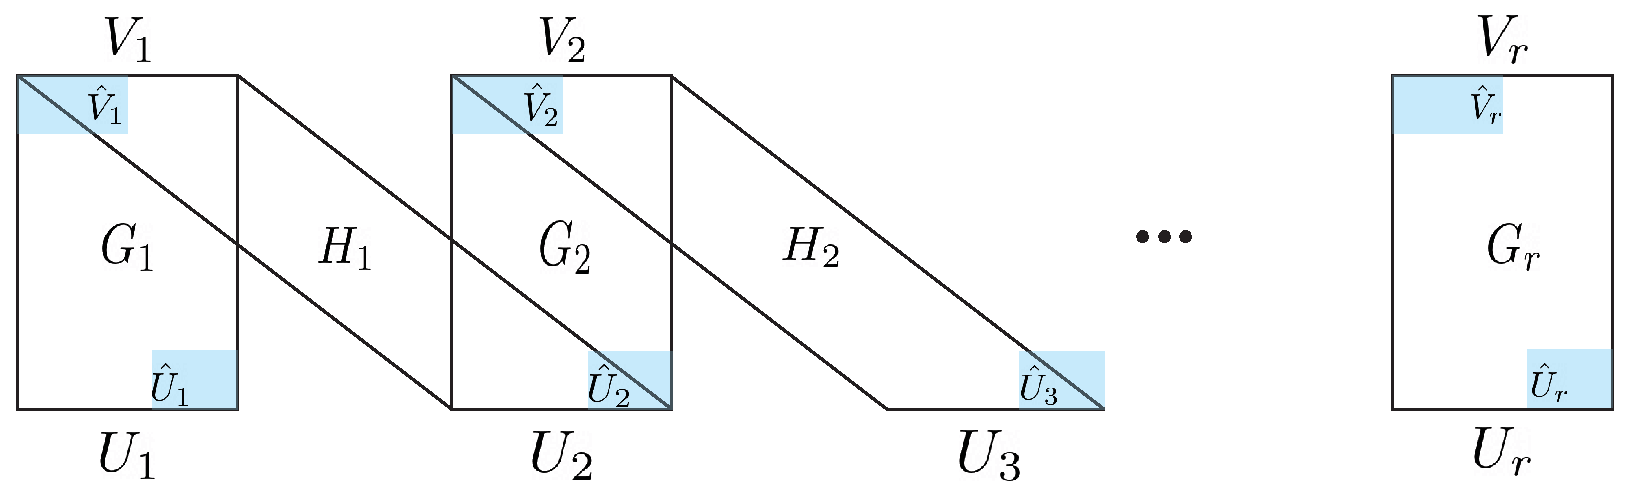
\includegraphics[scale=0.55]{fig/hardness.pdf}
  \caption{Illustration of graph $G' = (V', U', E')$. Each $G_i$ is shown by a rectangle and each $H_i$ is shown by a parallelogram. Top and bottom horizontal lines illustrate $V_i$ and $U_i$. Blue highlighted parts represent the vertex cover of the graph.}\label{fig:hardness}
  \end{center}
\end{figure}


Before proving the main result of this section, we characterize some properties of the constructed graph $G'$.

\begin{claim}\label{clm:matching-new-graph}
$\mu(G') = r\cdot \mu(G)$.
\end{claim}
\begin{myproof}
First, since all graphs $\{G_i\}_{i=1}^r$ are the same as $G$ and are vertex-disjoint, if we consider the maximum matching of $G$ in each of the $r$ graphs, we will have a matching of size $r\cdot \mu(G)$. Thus, $\mu(G') \geq r\cdot \mu(G)$.

Let $\hat{V} \cup \hat{U}$ be the minimum vertex cover of $G$ such that $\hat{V} \in V$ and $\hat{U} \in U$. By K\"{o}nig's Theorem (\Cref{prop:konig}), we have $|\hat{V} \cup \hat{U}| = \mu(G)$. Now we show there exists a vertex cover of size $r\cdot \mu(G)$ for graph $G'$. Let $\hat{V}_i \in V_i$ (resp. $\hat{U}_i \in U_i$) be the copy of vertices $V$ (resp. $U$) in graph $G_i$. We claim $(\bigcup_{i=1}^r \hat{V}_i \cup \hat{U}_i)$ is a vertex cover for $G'$. If an edge is in $G_i$, then at least one of its endpoints is in $\hat{V}_i \cup \hat{U}_i$ since $\hat{V}_i \cup \hat{U}_i$ is a vertex cover of $G_i$. Moreover, by the construction, $\hat{V}_i \cup \hat{U}_{i+1}$ is a vertex cover of $H_i$. Hence, each edge of $H_i$ is also covered by the vertex cover. Therefore, since there exists a vertex cover of size $|(\bigcup_{i=1}^r \hat{V}_i \cup \hat{U}_i)| = r\cdot |\hat{V} \cup \hat{U}| = r\cdot \mu(G)$, then we have $\mu(G') \leq r\cdot \mu(G)$ which completes the proof.
\end{myproof}

\begin{observation}\label{obs:path-cover-to-matching}
It holds $(2r-1)\cdot\mu(G) \leq \rho(G') \leq 2r\cdot \mu(G)$.
\end{observation}
\begin{myproof}
Since the union of maximum matching of all graphs $\{G_i\}_{i=1}^r$ and $\{H_i\}_{i=1}^{r-1}$ creates a path cover, we get $(2r-1)\cdot\mu(G) \leq \rho(G')$. Futhermore, if there exists a path cover of size larger than $2r\cdot \mu(G)$, then the maximum matching of these paths will be larger than $r\cdot \mu(G)$ which contradicts \Cref{clm:matching-new-graph}. Thus, $\rho(G') \leq 2r\cdot \mu(G)$.
\end{myproof}

Now we are ready to show the reduction.

\begin{lemma}
For any constant $\alpha > 0$, if there exists an algorithm that can estimate the maximum path cover within a $(\frac{1}{2} + \alpha)$-factor in $O(T(n))$ time, then the same algorithm can be used to estimate the maximum matching of bipartite graph $G$ within a $(1 - \epsilon)\cdot (\frac{1}{2} + \alpha)$-factor in $O(T(n/\epsilon))$ time.
\end{lemma}
\begin{myproof}
We construct graph $G'$ as described at the beginning of the section with $r = \frac{1}{2\epsilon}$. By \Cref{obs:path-cover-to-matching}, $(\frac{1}{\epsilon}-1)\cdot\mu(G) \leq \rho(G') \leq \frac{1}{\epsilon}\cdot \mu(G)$. Let $\tilde{\rho}$ be the estimate of the algorithm for the maximum path cover of $G'$. Hence, we have 
\begin{align*}
    (\frac{1}{2} + \alpha)(\frac{1}{\epsilon}-1)\cdot\mu(G) \leq \tilde{\rho} \leq \frac{1}{\epsilon}\cdot \mu(G).
\end{align*}
Now let $\tilde{\mu} = \epsilon\cdot\tilde{\rho}$ be the estimate for the maximum matching of $G$. Hence, 
\begin{align*}
    (1-\epsilon)(\frac{1}{2} + \alpha)\cdot\mu(G) \leq \tilde{\mu} \leq \mu(G).
\end{align*}
Since the number of vertices and number of edges of $G'$ is $r=\frac{1}{2\epsilon}$ times more than $G$, then the running time will be $O(T(n/\epsilon))$.
\end{myproof}


A reduction to matchings can also be proved for $(1,2)$-TSP, albeit with an extra promise for the matching instance that the matching is either perfect or half-perfect. This problem, formalized below, also remains open in the study matchings. We show that a better than $1.5$-approximation for $(1,2)$-TSP in $\widetilde{O}(n)$ time would resolve this question.

\begin{problem}\label{problem:matching-promised}
Suppose that we are given a bipartite graph $G=(L, R, E)$ with $|L| = |R| = n$ and are promised that either $\mu(G) = n$ or $\mu(G) = (\frac{1}{2}+\epsilon)n/2$ for any desirably small constant $\epsilon > 0$. Provided adjacency matrix access to the graph, does there exist an $n^{1+o(1)}$ time algorithm that distinguishes the two?
\end{problem}

\begin{theorem}\label{cor:matching-via-12tsp}
    If there is an algorithm that estimates the size of $(1,2)$-TSP within a $(\frac{3}{2} - \epsilon_0)$-factor for some fixed constant $\epsilon_0 \in (0, \frac{1}{4}]$ in $n^{1+o(1)}$, then \cref{problem:matching-promised} can indeed be solved in $n^{1+o(1)}$ time.
\end{theorem}
\begin{myproof}
Let $G_1$ and $G_2$ be two graphs with $n$ vertices such that $\mu(G_1) = n$ and $\mu(G_2) = (\frac{1}{2} + \frac{\epsilon_0}{16})$. We construct graph $G_1' = (V_1', E_1')$ and $G_2' = (V_2', E_2')$ as described at the beginning of the section with $r = \frac{1}{\epsilon_0}$. By \Cref{obs:path-cover-to-matching}, we have $\rho(G_1') \geq (\frac{2}{\epsilon_0} - 1)n$ and $\rho(G_2') \leq (\frac{1}{\epsilon_0}  + \frac{1}{8})n$. Thus, by \Cref{obs: bounding-TSP-with-DP}, we get
\begin{align*}
    \tspsize{V_1'} \leq \frac{4}{\epsilon_0}n - (\frac{2}{\epsilon_0} - 1)n = (\frac{2}{\epsilon_0} + 1)n,\\
    \tspsize{V_2'} \geq \frac{4}{\epsilon_0}n - (\frac{1}{\epsilon_0} + \frac{1}{8})n - 1 \geq (\frac{3}{\epsilon_0} - \frac{1}{4})n,
\end{align*}
for sufficiently large $n$, which implies
\begin{align*}
    \frac{\tspsize{V_2'}}{\tspsize{V_1}} = \frac{3 - \epsilon_0/4}{2 + \epsilon_0} \geq \frac{3}{2} - \epsilon_0.
\end{align*}
Therefore, the algorithm for (1,2)-TSP can distinguish between $G_1'$ and $G_2'$ which implies \cref{problem:matching-promised} can be solved in $n^{1+o(1)}$ time for $\epsilon = \epsilon_0/16$.
\end{myproof}


\paragraph{Lower Bound for Graphic TSP:} note that we can reduce an instance of (1,2)-TSP to graphic TSP by adding a new vertex and connecting the newly added vertex to all vertices of the graph. Therefore, the $n^{1+o(1)}$ time lower bound also holds for graphic TSP.


\subsection{Information-Theoretic Lower Bounds on the Running Time}\label{sec:hardness}
Since any constant approximation algorithm for estimating maximum path cover can be used to estimate the size of matching within a constant factor, then all of the lower bounds for $O(1)$-approximating maximum matching in sublinear time also hold for $(1)$-approximating maximum path cover in sublinear time. We restate some of these lower bounds along with a short proof (see \cite{behnezhad2021} for a detailed discussion).

\begin{lemma}\label{lem:hardness-adjacency-list}
Any algorithm that estimates maximum path cover within a constant multiplicative factor requires $\Omega(n)$ queries in the adjacency list model.
\end{lemma}
\begin{myproof}
Consider two graphs that the first one does not have any edge and the second one has only a single edge. In order to give any multiplicative approximation for maximum path cover, the algorithm needs to find the edge which requires $\Omega(n)$ queries in the adjacency list model. 
\end{myproof}

\begin{lemma}
Any algorithm that estimates maximum path cover within a constant multiplicative factor require $\Omega(n^2)$ queries in the adjacency matrix model.
\end{lemma}
\begin{myproof}
Consider the same construction as \Cref{lem:hardness-adjacency-list}. To give any multiplicative approximation for maximum path cover, the algorithm needs to find the edge which requires $\Omega(n^2)$ queries in the adjacency matrix model. 
\end{myproof}


\begin{lemma}
Any algorithm that estimates maximum path cover within a multiplicative-additive  requires $\Omega(n)$ queries in the adjacency matrix model.
\end{lemma}
\begin{myproof}
Consider a graph with no edge and a graph with one Hamiltonian cycle and no other edges. In order for the algorithm to distinguish between these two graphs, it must find at least one edge of the second graph which requires $\Omega(n)$ queries in the adjacency matrix model. 
\end{myproof}

There is also a lower bound for multiplicative-additive estimation of matching in adjacency list model \cite{PARNAS2007183} that also holds for maximum path cover.

\begin{lemma}
Any algorithm that estimates maximum path cover within a constant multiplicative-additive factor requires $\Omega(\bar{d})$ queries in the adjacency list model.
\end{lemma}




\paragraph{Acknowledgements.} Mohammad Roghani and Amin Saberi were supported by NSF award 1812919 and ONR award 141912550. Soheil Behnezhad and Aviad Rubinstein were supported by NSF CCF-1954927, and a David and Lucile Packard Fellowship. Soheil Behnezhad was additionally supported by NSF Awards 1942123, 1812919 and by Moses Charikar's Simons Investigator Award.